\chapter{Algoritmos exactos para \problem{STAR ROUTING}}
\label{ch:exactos}

En este cap'itulo proponemos dos algoritmos exactos para \problem{SR} general. Comenzamos el cap'itulo introduciendo el concepto de \textit{funci'on de acotaci'on}, que nos permitir'a acortar la ejecuci'on de los algoritmos exactos.

\section{Funciones de acotaci'on}

Los algoritmos exactos para problemas combinatorios suelen utilizar t'ecnicas como backtracking. En este tipo de algoritmos la construcci'on de una solución suele ser un proceso ordenado que mantiene una soluci'on parcial o incompleta, y en cada paso agrega alg'un elemento a la misma. Supongamos que estamos en el medio de la construcci'on de una soluci'on para una instancia $(G, X)$ de \problem{SR}. M'as espec'ificamente, supongamos que ya constru'imos un camino $P$ que cubre algunos de los clientes $X$. Nos interesa tener una cota inferior sobre cu'anto nos costar'ia, en longitud, extender $P$ a una soluci'on factible de esta instancia de \problem{SR}.

Usualmente, una funci'on de acotaci'on se definir'ia en este caso como una funci'on $B$ definida para cada camino $P$ del grafo de una instancia arbitraria $(G, X)$ de \problem{SR}, tal que $B(P)$ es una cota inferior para el costo, en longitud, de extender $P$ a una soluci'on factible de $(G, X)$. Vale notar que en nuestro caso, una funci'on de acotaci'on $B(P)$ depende, en general, s'olo del 'ultimo v'ertice de $P$ y del conjunto de clientes que quedan por cubrir. Teniendo en cuenta esto, utilizamos una definici'on alternativa de este concepto, para que la funci'on s'olo dependa de un v'ertice y un subconjunto de aristas, y no de todo un camino. Esto tiene la ventaja de hacer m'as clara la notaci'on, al concentrarse s'olo en los elementos relevantes que intervienen en la funci'on de acotaci'on (y esto, a su vez, facilita el trabajo de idear funciones de acotaci'on).

\begin{definition}
Sea $(G, X)$ una instancia de \problem{SR}. Una \textit{funci'on de acotaci'on} es una funci'on $B$ definida para cada v'ertice $u$ y cada subconjunto de aristas $F$ de $X$, tal que $B(u, F)$ es una cota inferior para la longitud de una soluci'on 'optima de \problem{s-SR} para $(G, F, u)$.
\end{definition}

\noindent
A veces una funci'on de acotaci'on s'olo depende de $F$, en cuyo caso omitimos el argumento $u$.

Notar que $\problem{s-SR}^*(G, F, u) \geq \problem{SR}^*(G, F)$ para todo $F$ y $u$, pues \problem{SR} admite soluciones factibles que empiezan en cualquier v'ertice, inclusive en $u$. Luego, si $\problem{SR}^*(G, F) \geq B(F)$ para todo $F$, entonces $B$ es una funci'on de acotaci'on. Esto indica que podemos buscar funciones de acotaci'on pensando en cotas inferiores para la soluci'on 'optima de una instancia $(G, F)$ de \problem{SR}.

Rec'iprocamente, supongamos que tenemos una cota $B(u, F)$. Observemos que siempre existe un v'ertice $u_0$ tal que $\problem{SR}^*(G, F) = \problem{s-SR}^*(G, F, u_0)$. Luego, $\problem{SR}^*(G, F) \geq B(u_0, F)$, lo cual nos da una cota inferior para $\problem{SR}^*(G, F)$. Por lo tanto, a partir de una cota podemos obtener una cota inferior para \problem{SR}.

Durante el resto del cap'itulo, frecuentemente diremos \textit{cota} en lugar de \textit{funci'on de acotaci'on}. A continuaci'on presentamos varias cotas, las cuales hemos clasificado en distintas clases, utilizando como criterio la similitud entre ellas.

\subsection{Cotas con cubrimientos de v'ertices}

Las siguientes cotas involucran el concepto de vertex cover m'inimo.

\begin{theorem}
\label{th:cota_vc}
$B(F) = \tau(G[F]) - 1$ es una cota.
\begin{proof}
El conjunto de v'ertices de cualquier soluci'on factible $P$ de \problem{SR} para $G$ y $F$, contiene un cubrimiento de v'ertices de $G[F]$, con lo cual $|P| \geq \tau(G[F])$. Luego, si adem'as $P$ es 'optimo, tenemos $\problem{SR}^*(G, F) = \length(P) = |P| - 1 \geq \tau(G[F]) - 1$.
\end{proof}
\end{theorem}

\begin{corollary}
\label{co:sr_tau}
$\problem{SR}^*(G, X) \geq \tau(G[X]) - 1$
\end{corollary}

Puesto que utilizaremos a las cotas como parte de un algoritmo exacto, es de nuestro inter'es que su c'omputo sea eficiente. En el caso general, no sabemos computar la cota del \autoref{th:cota_vc} en tiempo polinomial, pues \problem{VC} es \class{NP-completo} \cite{Ka72}, aunque s'i podemos hacerlo si $G$ es un grafo grilla, pues en este caso $G$ es bipartito, al igual que $G[F]$, por lo que podemos calcular $\tau(G[F])$ eficientemente, como indica el \autoref{th:vc_sobre_bipartitos_es_polinomial}. De todos modos, no todo est'a perdido en el caso general. Como cualquier cota inferior sobre $\tau(G[F])$ nos da una nueva cota, si encontramos una buena cota inferior computable en tiempo polinomial, habremos obtenido una funci'on de acotaci'on polinomial. El siguiente lema exhibe dos posibles cotas inferiores, una de las cuales vale para grafos arbitrarios.

\begin{lemma}
Sea $H$ un grafo con $m$ aristas.
\begin{enumerate}
\item Si $H$ es un subgrafo de un grafo grilla, entonces $\tau(H) \geq \ceil{m / 4}$.
\item Sea $d_1 \geq \dots \geq d_n$ la secuencia de grados de $H$. Entonces $\tau(H) \geq \min\{\ell : d_1 + \dots + d_{\ell} \geq m\}$.
\end{enumerate}

\begin{proof}
\begin{enumerate}
\item Como $H$ es un subgrafo de un grafo grilla, cada v'ertice puede cubrir, como mucho, 4 aristas.

\item Notar que la cota $\tau(H) \geq \ceil{m / 4}$ sobrestima cu'anto es capaz de cubrir cada v'ertice de $H$. Podemos hacer una estimaci'on m'as precisa si tenemos en cuenta la secuencia de grados de $H$. Sea $d'_1 \geq \dots \geq d'_{\tau(H)}$ la secuencia de grados de un vertex cover m'inimo cualquiera de $H$. La secuencia $(d'_i)$ es una subsecuencia de $(d_i)$, y son ambas mon'otonas no crecientes, con lo cual es $d_i \geq d'_i$ para cada $1 \leq i \leq \tau(H)$. Por otro lado, como $(d'_i)$ proviene de un vertex cover de $H$, vale $\sum_{i = 1}^{\tau(H)} d'_i \geq m$. Entonces $\tau(H) \geq \min\{\ell: \sum_{i = 1}^{\ell} d'_i \geq m\}$. Usando que $d_i \geq d'_i$, es $\min\{\ell : \sum_{i = 1}^{\ell} d'_i \geq m\} \geq \min\{\ell : \sum_{i = 1}^{\ell} d_i \geq m\}$. Por transitividad, llegamos a la desigualdad buscada.
\end{enumerate}
\end{proof}
\end{lemma}

\begin{corollary}
\hfill
\begin{enumerate}
\item Si $G$ es un grafo grilla, entonces $B(F) = \ceil{|F|/4} - 1$ es una cota.
\item Sea $d_1 \geq \dots \geq d_n$ la secuencia de grados de $G[F]$. Entonces $B(F) = \min\{\ell : d_1 + \dots + d_{\ell} \geq |F|\} - 1$ es una cota.
\end{enumerate}
\end{corollary}

\subsection{Cotas con distancias}

Las siguientes cotas involucran el c'omputo de distancias entre v'ertices y aristas, y entre pares de aristas. Primero, debemos introducir estas nociones de distancias.

\begin{definition}[Distancia entre aristas]
\label{de:dist_aristas}
Dadas dos aristas $e$ y $f$ de un grafo, definimos $\dist(e, f)$ como la distancia m'as peque\~na entre un extremo de $e$ y uno de $f$. Esto es,

\[\dist(e, f) = \min\limits_{\substack{u \text{ extremo de }e \\ v \text{ extremo de }f}} \dist(u, v)\]
\end{definition}

\begin{definition}
Sean $e$ una arista y $v$ un v'ertice de un grafo. Se define

\[\dist(e, v) = \dist(v, e) = \min\limits_{u \text{ extremo de }e} \dist(u, v)\]
\end{definition}

\begin{theorem}
\label{th:cota_dist_x2}
$B(u, F) = \max\limits_{\{e, f\} \subseteq F} (\min(\dist(u, e), \dist(u, f)) + \dist(e, f))$ es una cota.

\begin{proof}
Tomemos dos aristas arbitrarias $e, f \in F$. Cualquier camino desde $u$ que las cubra visitar'a a una de las dos en primer lugar (en caso de que ambas aristas sean cubiertas por primera vez por el mismo v'ertice, tomamos cualquiera de $e$ o $f$). Desde $u$ hasta ese punto, el camino tendr'a longitud, al menos, $\min(\dist(u,e), \dist(u, f))$. Luego de eso, el camino eventualmente llegar'a a la segunda arista. La distancia recorrida entre ellos ser'a al menos $\dist(e, f)$. En total, el camino tendr'a longitud al menos $\min(\dist(u,e), \dist(u, f)) + \dist(e, f)$. Como $e$ y $f$ son cualesquiera, podemos tomar el m'aximo valor de esta longitud, sobre todos los $e$ y $f$ (es decir, nos quedamos con la mejor cota).
\end{proof}
\end{theorem}

Notemos que esta cota calcula cu'al de los recorridos $u \rightsquigarrow e \rightsquigarrow f$ o $u \rightsquigarrow f \rightsquigarrow e$ es m'as corto, para cada par de aristas $e, f \in F$. 'Esto se generaliza en forma natural a m'as de dos aristas de $F$.

\begin{theorem}
\label{th:cota_dist_x3}
\begin{align*}
B(u, F) = \max\limits_{\{e, f, g\} \subseteq F} \min\{
&\dist(u, e) + \dist(e, f) + \dist(f, g),\\
&\dist(u, e) + \dist(e, g) + \dist(g, f),\\
&\dist(u, f) + \dist(f, e) + \dist(e, g),\\
&\dist(u, f) + \dist(f, g) + \dist(g, e),\\
&\dist(u, g) + \dist(g, e) + \dist(e, f),\\
&\dist(u, g) + \dist(g, f) + \dist(f, e)\}
\end{align*}
es una cota.
\end{theorem}

Las siguiente cota es una especie de generalizaci'on de las dos anteriores, pero que no involucra un v'ertice $u$.

\begin{theorem}
$B(F) = \problem{PTSP}^*(K(F), \dist)$ es una cota.
\end{theorem}

Intuitivamente, esta cota es v'alida porque un camino que cubre un conjunto de clientes $F$ puede pensarse como un camino en el grafo completo $K(F)$. La demostraci'on se sigue directamente del \autoref{th:clients_bounds}. No la hacemos aqu'i porque utiliza un concepto que a'un no hemos introducido (el de conjunto de permutaciones de clientes asociadas a un camino, que se presenta en el \autoref{ch:exactos}).

Como sucedi'o antes, no sabemos computar esta cota en tiempo polinomial. En este caso, utilizamos la cota inferior $\problem{PTSP}^*(K(F), \dist) \geq \mst(K(F), \dist)$, que s'i sabemos computar eficientemente.

\begin{corollary}
\label{co:cota_mst}
$B(F) = \mst(K(F), \dist)$ es una cota.

\begin{proof}
Una soluci'on factible de \problem{PTSP} es un camino hamiltoniano, y un camino hamiltoniano es un 'arbol generador. Luego, toda soluci'on factible tiene peso mayor o igual al peso de un 'arbol generador m'inimo.
\end{proof}
\end{corollary}

\subsection{Cotas combinadas}

Las siguientes cotas combinan el concepto de vertex cover m'inimo con el de distancias.

\begin{definition}
Sean $H_1$ y $H_2$ subgrafos de un grafo. Se define

\[\dist(H_1, H_2) = \min\limits_{\substack{u_1 \in V(H_1) \\ u_2 \in V(H_2)}} \dist(u_1, u_2)\]
\end{definition}

\begin{theorem}
Sean $H_1, \dots, H_r$ las componentes conexas de $G[F]$. Sea $H = K(\{H_1, \dots, H_r\})$. Entonces $B(F) = \tau(G[F]) - 1 + \problem{PTSP}^*(H, \dist) - (r - 1)$ es una cota.

\begin{proof}
Sea $P$ una soluci'on 'optima de \problem{SR} para $(G, F)$. El camino $P$ cubre cada arista de cada $H_i$. M'as a'un, cada v'ertice de $P$ s'olo puede cubrir aristas de s'olo una componente $H_i$. Luego, $P$ usa al menos

\begin{equation}
\label{eq:1}
\sum_{i = 1}^r\tau(H_i) = \tau(G[F])
\end{equation}

\noindent
v'ertices para cubrir las aristas de las componentes conexas de $G[F]$.

Adem'as de estos v'ertices que cubren las componentes, $P$ recorre v'ertices intermedios, que no pertenecen a ning'un $H_i$. A continuaci'on, acotamos esta cantidad. Sean $i_1, \dots, i_s$ tales que $H_{i_j}$ es el $j$-'esimo subgrafo que visita $P$ en su recorrido. Esto significa que $P$ primero visita $H_{i_1}$, recorre algunos de sus v'ertices y eventualmente se va, para dirigirse hacia $H_{i_2}$. As'i sucesivamente. Notar que una componente conexa podr'ia ser visitada varias veces, as'i que podr'ia aparecer varias veces en la secuencia.

Entre $H_{i_j}$ y $H_{i_{j + 1}}$ hay al menos $\dist(H_{i_j}, H_{i_{j + 1}}) - 1$ v'ertices que no pertenecen a ninguna componente. Por ende, en total hay al menos $\sum_{j = 1}^{s - 1} (\dist(H_{i_j}, H_{i_{j + 1}}) - 1)$ v'ertices de $P$ que no pertenecen a ninguna componente de $G[F]$. Como $\langle H_{i_1}, \dots, H_{i_s} \rangle$ es un camino de $H$ que recorre todos sus v'ertices, y $H$ es completo, podemos extraerle un camino hamiltoniano de $H$. Teniendo en cuenta este camino hamiltoniano, separamos los t'erminos de la suma $\sum_{j = 1}^{s - 1} (\dist(H_{i_j}, H_{i_{j + 1}}) - 1)$ en dos, seg'un la arista $\{H_{i_j}, H_{i_{j + 1}}\}$ forme parte del camino hamiltoniano, o no. Hay $r - 1$ t'erminos correspondientes a aristas que est'an en el camino hamiltoniano, y suman al menos $\problem{PTSP}^*(H, \dist) - (r - 1)$, . Los dem'as t'erminos suman una cantidad no negativa. Entonces

\begin{equation}
\label{eq:2}
\sum_{j = 1}^{s - 1} (\dist(H_{i_j}, H_{i_{j + 1}}) - 1) \geq \problem{PTSP}^*(H, \dist) - (r - 1)
\end{equation}

Como los v'ertices contados en \eqref{eq:1} y \eqref{eq:2} son disjuntos, $P$ tiene al menos tantos v'ertices como la suma de esas cantidades. Luego

\[\problem{SR}^*(G, F) = \length(P) = |P| - 1 \geq \tau(G[F]) - 1 + \problem{PTSP}^*(H, \dist) - (r - 1)\]

\noindent
como quer'iamos probar.

\end{proof}
\end{theorem}

Notar que como $\problem{PTSP}^*(H, \dist) \geq r - 1$, esta cota es una generalizaci'on de la cota del \autoref{th:cota_vc}. Como ya hicimos antes, el siguiente corolario acota \problem{PTSP} por \mst.

\begin{corollary}
\label{co:cota_vc_mst}
$B(F) = \tau(G[F]) - 1 + \mst(H, \dist) - (r - 1)$ es una cota.
\end{corollary}

En el caso en que $G$ es grilla, podremos computar esta nueva cota en tiempo polinomial. En el caso general, la cota sigue siendo exponencial, y debemos utilizar una cota inferior polinomial para $\tau(G[F])$.

\subsection{Otras cotas}

La 'ultima cota que presentamos no encaja en ninguna de las categor'ias anteriores.

\begin{theorem}
\label{th:cota_clients_count}
Si $G$ es un grafo grilla, entonces $B(F) = \floor{|F| / 3} - 1$ es una cota.

\begin{proof}
Llamemos $M(k)$ al m'inimo valor de una soluci'on 'optima de SR para una instancia con $k$ clientes, es decir,
\[M(k) = \min \{\problem{SR}^*(G, F) : (G, F) \text{ es una instancia de \problem{SR} sobre grillas con }|F| = k\}\]

\noindent
Se tiene $\problem{SR}^*(G, F) \geq M(|F|)$, con lo cual toda cota inferior de $M(|F|)$ nos da una cota para \problem{SR}. El resto de la demostraci'on consiste en probar que $M(k) \geq \floor{k / 3} - 1$.

Si $k < 3$, el resultado es trivial. Sea $k \geq 3$. Construiremos un conjunto de aristas $F_k$, pertenecientes a un grafo grilla (no importa cu'al), tal que $M(k) = \problem{SR}^*(-, F_k)$, al mismo tiempo que probamos que $\problem{SR}^*(-, F_k) \geq \floor{k / 3} - 1$.

Para ganar intuici'on sobre la forma de $F_k$, consideramos el conjunto de clientes de la \autoref{fig:exactos_1}. Veamos que el camino indicado con flechas es una soluci'on 'optima de \problem{SR} para esos clientes. El primer v'ertice cubre 4 clientes, y los restantes cubren 3 nuevos clientes cada uno. No hay otra forma de disponer esa misma cantidad de clientes, de modo tal que exista un camino m'as corto cubri'endolos a todos, puesto que cada v'ertice del camino maximiza la cantidad de \emph{nuevos} clientes que son cubiertos.

La demostraci'on es una generalizaci'on del ejemplo anterior. Primero, elegimos cierto conjunto $F_k$ de $k$ clientes, contenidos en un grafo grilla, y consideramos un camino $P$ que cubra $F_k$. Esto es, $P$ es una soluci'on factible de \problem{SR} para $(-, F_k)$. Luego, se prueba que \emph{cualquier} soluci'on factible de \emph{cualquier} instancia de \problem{SR} sobre grillas con $k$ clientes, tiene longitud mayor o igual a $\length(P)$. Esto implica que $\problem{SR}^*(-, F_k) = \length(P) \leq \problem{SR}^*(G, F)$ para toda instancia $(G, F)$ de \problem{SR} sobre grillas con $|F| = k$, de lo cual se deduce que $M(k) = \length(P)$.

Antes de continuar con la demostraci'on, introducimos un concepto que formaliza la noci'on de cantidad de nuevos clientes que se van cubriendo a lo largo de un camino. Dado un grafo $G$, un subconjunto de aristas $F$ de $G$, y un camino $P = \langle u_1, \dots, u_r \rangle$ de $G$, la \textit{secuencia de cobertura de $P$ para $F$} es la secuencia de n'umeros $a_1, \dots, a_r$, tal que si recorremos a $P$ de principio a fin, $a_i$ es el n'umero de aristas de $F$ que son cubiertos por $u_i$, y que no son cubiertos por ninguno de $u_1, \dots, u_{i - 1}$.

\begin{figure}[h]
	\begin{center}
		\input{img/exactos_1.pdf_tex}
	\end{center}		
	\caption{$F_k$ con $k = 13$.}
	\label{fig:exactos_1}
\end{figure}

Consideramos tres casos, dependiendo del resto m'odulo 3 de $k$. Esta divisi'on en casos se debe a que no siempre es posible disponer los clientes exactamente como en la \autoref{fig:exactos_1}.

\begin{figure}[h]
	\begin{center}
		\input{img/exactos_2.pdf_tex}
	\end{center}		
	\caption{$F_k$ con (a) $k = 3r$, (b) $k = 3r + 1$, (c) $k = 3r + 2$.}
	\label{fig:exactos_2}
\end{figure}

Si $k = 3r + 1$ para cierto $r$, elegimos $F_k$ como indica la \autoref{fig:exactos_2}-(b). Sea $P$ el camino indicado con flechas. La secuencia de cobertura de $P$ para $F_k$ es $4, \underbrace{3, \dots, 3}_{r - 1 \text{ veces}}$. Llamemos $a_1, \dots, a_r$ a esta secuencia. Sea $(G, F)$ una instancia arbitraria de \problem{SR} sobre grillas, y sea $Q$ una soluci'on factible de \problem{SR} para $(G, F)$. Sea $b_1, \dots, b_s$, con $s = |Q|$, su secuencia de cobertura para $F$. Queremos ver que $\length(P) \leq \length(Q)$, o equivalentemente $r \leq s$.

Notar que $b_i \leq 4$ para todo $i$, puesto que $G$ es un grafo grilla. Adem'as $b_i \leq 3$ si $i > 1$, dado que un v'ertice puede cubrir s'olo 4 clientes si y s'olo si es el primer v'ertice en un camino y est'a rodeado por 4 clientes. Todo otro v'ertice distinto del primero no puede cubrir 4 nuevos clientes, puesto que el v'ertice previo en el camino tuvo que haber cubierto alguno de los cuatro clientes incidentes. Entonces, tenemos que $b_i \leq a_i$ para todo $1 \leq i \leq \min\{r, s\}$. Como adem'as las sumas $\sum_{i = 1}^r a_i$ y $\sum_{i = 1}^s b_i$ son iguales (a $k$), debe ser $r \leq s$, como quer'iamos.

En definitiva, si $k = 3r + 1$, es $M(k) = \length(P) = r - 1 = \floor{k / 3} - 1$. Resta probar la desigualdad para $k = 3r$ y $k = 3r + 2$. Para $k = 3r + 2$ elegimos $F_k$ como indica la \autoref{fig:exactos_2}-(c). El camino indicado $P$ tiene secuencia de cobertura $4, \underbrace{3, \dots, 3}_{r - 1\text{ veces}}, 1$, y se puede probar, igual que en el caso anterior, que es igual o m'as corto que cualquier soluci'on factible de cualquier instancia sobre grillas con $k$ clientes. En este caso, tenemos $\length(P) = r$, de modo que $M(k) = \length(P) = r = \floor{k / 3}$ que obviamente cumple la desigualdad.

Finalmente, para $k = 3r$ consideramos el conjunto de clientes indicado en la \autoref{fig:exactos_2}-(a). El camino considerado tiene longitud $r - 1$, obteni'endose tambi'en la desigualdad buscada.
\end{proof}
\end{theorem}

\begin{corollary}
\label{co:sr_floor}
Si $G$ es un grafo grilla, $\problem{SR}^*(G, X) \geq \floor{|X| / 3|} - 1$.
\end{corollary}

\section{Algoritmos exactos}

En esta sección presentamos dos algoritmos exactos para SR: uno basado en la técnica de \emph{backtracking} y otro en la de \emph{programación dinámica}. A lo largo de la sección consideraremos una instancia arbitraria $(G, X)$ de SR y llamamos $k = |X|$ a la cantidad de clientes de la misma.

\subsection{Algoritmo de backtracking}

El algoritmo de backtracking que proponemos considera todas las posibles permutaciones de las aristas de $X$. La idea detr'as de esto es que toda soluci'on factible de \problem{SR} cubre los clientes en cierto orden. El algoritmo produce todos esos ordenamientos, ya que alguno de ellos corresponde al orden en que alguna soluci'on 'optima visita las aristas. Surgen algunos interrogantes, que iremos respondiendo. ?`Dada una soluci'on factible, cu'al es el orden en que se cubren los clientes? ?`Es 'unico este orden?

\begin{definition}
\label{de:conjunto_de_permutaciones}
Sea $F$ un subconjunto de aristas de $G$. Sea $P = \langle u_1, \dots, u_r \rangle$ un camino de $G$ que cubre $F$. Definimos el \textit{conjunto de permutaciones de $F$ asociadas a $P$}, y lo notamos $\Pi(F, P)$, del siguiente modo. Una permutaci'on $\langle e_1, \dots, e_{\ell} \rangle$ de $F$ pertenece a $\Pi(F, P)$ si existe una funci'on mon'otona no decreciente $f: \{1, \dots, \ell\} \to \{1, \dots, r\}$ tal que $u_{f(i)}$ cubre a $e_i$, para cada $1 \leq i \leq \ell$.
\end{definition}

\noindent
Intuitivamente, $\pi \in \Pi(F, P)$ si $P$ puede cubrir $F$ en el orden dado por $\pi$.

%\begin{lemma}
%Supongamos que $G$ es un grafo grilla. Sea $P$ una soluci'on factible de \problem{SR}. Sea $\langle e_1, \dots, e_k \rangle \in \Pi(P)$, y $f$ una funci'on asociada a esta permutaci'on. Sea $Q$ un camino de $G$ que se define del siguiente modo.
%para la soluci'on 'optima de una instancia $(G, F)$ de \problem{SR}.

%\begin{enumerate}
%	\item Definimos v'ertices $v_1, \dots, v_k$ inductivamente, del siguiente modo. Definimos $v_1 = u_{f(1)}$. Supongamos ya elegidos $v_1, \dots, v_i$. Elegimos $v_{i + 1}$ de modo tal que $\dist(v_i, e_{i + 1}) = \dist(v_i, v_{i + 1})$. En otras palabras, $v_{i + 1}$ es el extremo de $e_{i + 1}$ m'as cercano a $v_i$.
%	\item Sea $Q_i$ un camino m'inimo entre $v_i$ y $v_{i + 1}$.
%	\item Definimos $Q = Q_1 \circ \dots \circ Q_{k - 1}$.
%\end{enumerate}
%
%\noindent
%Entonces $Q$ es una soluci'on factible de \problem{SR} para $(G, X)$ tal que $\length(Q) \leq \length(P)$.
%
%\begin{proof}
%Es una soluci'on factible porque, por construcci'on, es un camino de $G$ y cubre cada $e_i$. Veamos que tiene longitud no mayor que $\length(P)$.
%
%Para empezar, notemos que $\length(Q) = \sum_{j = 1}^{k - 1} \length(Q_i) = \sum_{j = 1}^{k - 1} \dist(v_j, v_{j + 1})$.
%
%\begin{claim}
%Para cada $1 \leq i < k$, vale
%
%\[\sum_{j = 1}^i \dist(v_j, v_{j + 1}) \leq \sum_{j = 1}^i \dist(u_{f(j)}, u_{f(j + 1)})\]
%
%\noindent
%M'as a'un, si $v_{i + 1} \neq u_{f(i + 1)}$, la desigualdad es estricta.
%
%\begin{proof}
%Escribamos $A_i = \sum_{j = 1}^i \dist(v_j, v_{j + 1})$ y $B_i = \sum_{j = 1}^i \dist(u_{f(j)}, u_{f(j + 1)})$. Hacemos inducci'on sobre $i$. El caso base es
%
%\begin{align*}
%A_1 = \dist(v_1, v_2) &= \dist(v_1, e_2) & \text{(definici'on de } v_2 \text{)}\\
%&\leq \dist(u_{f(1)}, e_2) & \text{(} v_1 = u_{f(1)} \text{)}\\
%&\leq \dist(u_{f(1)}, u_{f(2)}) = B_1 & \text{(} u_{f(2)} \text{ es extremo de } e_2 \text{)}
%\end{align*}
%
%Asumamos que la afirmaci'on vale para $i$, y veamos que es cierta para $i + 1$. Es $A_{i + 1} = A_i + \dist(v_{i + 1}, v_{i + 2})$. Separamos en casos, y acotamos los t'erminos $A_i$ y $\dist(v_{i + 1}, v_{i + 2})$ por separado.
%
%\begin{itemize}
%\item $v_{i + 2} = u_{f(i + 2)}$
%	\begin{itemize}
%	\item $v_{i + 1} = u_{f(i + 1)}$
%	
%	Por hip'otesis inductiva, es $A_i \leq B_i$. Adem'as,  $\dist(v_{i + 1}, v_{i + 2}) = \dist(u_{f(i + 1)}, u_{f(i + 2)})$. Luego
%	
%	\begin{align*}
%	A_{i + 1} &= A_i + \dist(v_{i + 1}, v_{i + 2})\\
%	&\leq B_i + \dist(u_{f(i + 1)}, u_{f(i + 2)})\\
%	&= B_{i + 1}
%	\end{align*}
%
%	\item $v_{i + 1} \neq u_{f(i + 1)}$
%	
%	Por hip'otesis inductiva, es $A_i < B_i$. Como ambos valores son enteros, podemos decir que, m'as a'un, $A_i \leq B_i - 1$. Por otro lado,
%	
%	\begin{align*}
%	\dist(v_{i + 1}, v_{i + 2}) &= \dist(v_{i + 1}, u_{f(i + 2)})\\
%	&\leq \dist(v_{i + 1}, u_{f(i + 1)}) + \dist(u_{f(i + 1)}, u_{f(i + 2)})\\
%	&= 1 + \dist(u_{f(i + 1)}, u_{f(i + 2)})
%	\end{align*}
%	
%	Luego,
%	
%	\begin{align*}
%	A_{i + 1} &= A_i + \dist(v_{i + 1}, v_{i + 2})\\
%	&\leq (B_i - 1) + (1 + \dist(u_{f(i + 1)}, u_{f(i + 2)}))\\
%	&= B_i + \dist(u_{f(i + 1)}, u_{f(i + 2)})\\
%	&= B_{i + 1}
%	\end{align*}
%	\end{itemize}
%
%\item $v_{i + 2} \neq u_{f(i + 2)}$
%	
%	\begin{itemize}
%	\item $v_{i + 1} = u_{f(i + 1)}$
%	
%	Es $A_i \leq B_i$. Como $u_{f(i + 2)}$ es el extremo de $e_{i + 2}$ m'as lejano a $v_{i + 1}$, y $G$ es una grilla, entonces
%	
%	\begin{align*}
%	\dist(v_{i + 1}, v_{i + 2}) &\leq \dist(v_{i + 1}, u_{f(i + 2)}) - 1 & \\
%	&= \dist(u_{f(i + 1)}, u_{f(i + 2)}) - 1 & \text{(} v_{i + 1} = u_{f(i + 1)} \text{)}
%	\end{align*}
%	
%	Luego,
%	
%	\begin{align*}
%	A_{i + 1} &= A_i + \dist(v_{i + 1}, v_{i + 2})\\
%	&\leq B_i + (\dist(u_{f(i + 1)}, u_{f(i + 2)}) - 1)\\
%	&= B_{i + 1} - 1\\
%	&< B_{i + 1}
%	\end{align*}
%	
%	\item $v_{i + 1} \neq u_{f(i + 1)}$
%	
%	Es $A_i \leq B_i - 1$. Como $v_{i + 2}$ es el extremo de $e_{i + 2}$ m'as cercano a $v_{i + 1}$, $v_{i + 1} \neq u_{f(i + 1)}$, $v_{i + 2} \neq u_{f(i + 2)}$, y $G$ es grilla, entonces $\dist(v_{i + 1}, v_{i + 2}) \leq \dist(u_{f(i + 1)}, u_{f(i + 2)})$. Por lo tanto,
%	
%	\begin{align*}
%	A_{i + 1} &= A_i + \dist(v_{i + 1}, v_{i + 2})\\
%	&\leq (B_i - 1) + \dist(u_{f(i + 1)}, u_{f(i + 2)})\\
%	&= B_{i + 1} - 1\\
%	&< B_{i + 1}
%	\end{align*}
%	
%	\end{itemize}
%\end{itemize}
%\end{proof}
%\end{claim}
%
%Poniendo $i = k - 1$, concluimos que $\length(Q) = \sum_{j = 1}^{k - 1} \dist(v_j, v_{j + 1}) \leq \sum_{j = 1}^{k - 1} \dist(u_{f(j)}, u_{f(j + 1)})$. Para terminar la demostraci'on, probaremos que $\sum_{j = 1}^{k - 1} \dist(u_{f(j)}, u_{f(j + 1)}) \leq \length(P)$. La clave aqu'i es que $f$ es mon'otona creciente. Esto implica que $P_j = \langle u_{f(j)}, \dots, u_{f(j + 1)} \rangle$ es un subcamino de $P$, y que $P_i$ y $P_j$ son disjuntos en ejes, si $i \neq j$. Como $\dist(u_{f(j)}, u_{f(j + 1)}) \leq \length(P_j)$, concluimos que
%
%\[\sum_{j = 1}^{k - 1} \dist(u_{f(j)}, u_{f(j + 1)}) \leq \sum_{j = 1}^{k - 1} \length(P_j) \leq \length(P)\]
%
%\end{proof}
%\end{lemma}

Dada una permutaci'on $\pi = \langle e_1, \dots e_k \rangle$ de $X$, nos interesa saber cu'al es la m'inima longitud de un camino $P$ tal que $\pi \in \Pi(X, P)$. La llamaremos \textit{longitud m'inima de $\pi$}, y la notamos $L(\pi)$. Si no existe tal camino $P$, definimos $L(\pi) = \infty$. Antes de ver c'omo computar $L(\pi)$, motivemos la utilidad de este n'umero.

\begin{proposition}
\label{pr:pi}
$\Pi(F, P) \neq \emptyset$

\begin{proof}
Escribamos $P = \langle u_1, \dots, u_r \rangle$. Iterando, de principio a fin, sobre cada v'ertice $u_i$ de $P$, vamos enumerando las aristas de $F$ que son cubiertos por $u_i$ y que no hab'ian sido cubiertas a'un. Si $u_i$ cubre m'as de una nueva arista, las enumeramos en cualquier orden. Sea $\pi = \langle e_1, \dots, e_{\ell} \rangle$ el resultado de esta enumeraci'on. Observemos que toda arista de $F$ est'a en $\pi$, pues $P$ cubre $F$. Luego, $\pi$ es una permutaci'on de los aristas de $F$.

Para ver que $\pi \in \Pi(F, P)$, debemos encontrar una funci'on $f$ tal como indica la definici'on de $\Pi(F, P)$. Definimos, para cada $1 \leq i \leq \ell$, el n'umero $f(i)$ como el 'indice del primer v'ertice de $P$ que cubre $e_i$. Veamos que esta $f$ cumple las condiciones necesarias. Obviamente, $u_{f(i)}$ cubre $e_i$. Adem'as, como $\pi$ es resultado de ir enumerando las aristas exactamente cuando son cubiertos por primera vez por $P$, es $f(i) \leq f(i + 1)$.
\end{proof}
\end{proposition}

\begin{remark}
Si $P$ es una soluci'on factible de \problem{SR} para $(G, X)$ y $\pi \in \Pi(X, P)$, entonces $L(\pi) \leq \length(P)$.
\end{remark}

Diremos que una soluci'on factible $P$ de \problem{SR} para $(G, X)$ realiza $L(\pi)$, si $\pi \in \Pi(X, P)$ y $\length(P) = L(\pi)$.

\begin{lemma}
\label{le:pi_min}
Entre todas las permutaciones de $X$, sea $\pi_{\textnormal{min}}$ una tal que $L(\pi_{\textnormal{min}})$ es m'inimo. Sea $P$ una soluci'on factible de \problem{SR} para $(G, X)$, que realiza $L(\pi_{\textnormal{min}})$. Entonces $P$ es una soluci'on 'optima.

\begin{proof}
Sea $Q$ una soluci'on 'optima de \problem{SR} para $(G, X)$. Por la \autoref{pr:pi}, es $\Pi(X, Q) \neq \emptyset$, as'i que podemos tomar un elemento $\pi_{\textnormal{opt}} \in \Pi(X, Q)$, cualquiera. Se tiene $L(\pi_{\textnormal{min}}) \leq L(\pi_{\textnormal{opt}})$. Luego

\[\length(P) = L(\pi_{\textnormal{min}}) \leq L(\pi_{\textnormal{opt}}) \leq \length(Q)\]

\noindent
Como $P$ es una soluci'on factible, es $\length(Q) \leq \length(P)$. Luego, debe ser $\length(P) = \length(Q)$, o sea que $P$ es una soluci'on 'optima.
\end{proof}
\end{lemma}

\begin{corollary}
\label{co:sr_longitud_minima_permutacion}
$\problem{SR}^*(G, X) = \min \{L(\pi) : \pi \text{ permutaci'on de } X\}$
\end{corollary}

Estos resultados sugieren que podemos encontrar el valor de una soluci'on 'optima de \problem{SR} para $(G, X)$, buscando el m'inimo $L(\pi)$. Veamos c'omo calcular $L(\pi)$, dada una permutaci'on $\pi$. Escribamos $\pi = \langle e_1, \dots, e_k \rangle$. La \autoref{fig:exactos_5} ayuda a hacernos una idea gr'afica del problema que intentamos resolver. Los trazos en l'ineas punteadas representan un camino entre los correspondientes v'ertices. Intuitivamente, un camino $P$ es tal que $\pi \in \Pi(X, P)$ si y s'olo si recorre las l'ineas punteadas, pasando por cada $e_i$. Buscamos la m'inima longitud de un camino con estas caracter'isticas.

Durante el resto de este cap'itulo, asumimos que los dos extremos de toda arista $e$ est'an enumerados de cierta forma (es decir, que $e$ es un par ordenado de v'ertices), y los llamamos $e[1]$ y $e[2]$.

\begin{figure}[h]
	\begin{center}
		\input{img/exactos_5.pdf_tex}
	\end{center}		
	\caption{Calcular $L(\pi)$ puede pensarse como encontrar la m'inima longitud de un camino que recorre las l'ineas punteadas, pasando por cada $e_i$. (Notar que los extremos de las aristas $e_i$ no son necesariamente disjuntos, con lo cual algunos de los trazos punteados podr'ian tener longitud $0$.)}
	\label{fig:exactos_5}
\end{figure}

Fijada una permutaci'on $\pi = \langle e_1, \dots, e_k \rangle$ de $X$, llamamos $\pi_i = \langle e_1, \dots, e_i \rangle$ y $X_i = \{e_1, \dots, e_i\}$. Definimos

\begin{align*}
L_1(i) =& \text{ m'inima longitud de un camino } P \text{ tal que }\\
&\pi_i \in \Pi(X_i, P) \text{ y que termina en } e_{i}[1]
\end{align*}

\noindent
An'alogamente se define $L_2(i)$, que requiere que el camino $P$ termine en $e_{i}[2]$. Notemos que $L(\pi) = \min\{L_1(k), L_2(k)\}$ es el n'umero buscado. Es f'acil ver que $L_1(1) = 0$, pues el camino $\langle e_{1}[1] \rangle$ realiza el m'inimo. An'alogamente, $L_2(1) = 0$.

Diremos que un camino $P$ de $G$ que cubre $X_i$ realiza $L_j(i)$, si $\pi_i \in \Pi(X_i, P)$, $P$ termina en $e_{i}[j]$, y $\length(P) = L_j(i)$.

\begin{theorem}
\label{th:longitud_minima}
\[L_1(i) = \min\{L_1(i - 1) + \dist(e_{i - 1}[1], e_{i}[1]), L_2(i - 1) + \dist(e_{i - 1}[2], e_{i}[1])\}\]
\[L_2(i) = \min\{L_1(i - 1) + \dist(e_{i - 1}[1], e_{i}[2]), L_2(i - 1) + \dist(e_{i - 1}[2], e_{i}[2])\}\]

\begin{proof}
Probaremos la recurrencia para $L_1$; la de $L_2$ es an'aloga.

Sea $P = \langle u_1, \dots, u_r \rangle$ un camino que realiza $L_1(i)$. Como $\pi_i \in \Pi(X_i, P)$, existe una funci'on mon'otona no decreciente $f$ tal que $u_{f(j)}$ cubre $e_j$, para cada $1 \leq j \leq i$. Observemos que $r = f(i)$, pues como el subcamino $\langle u_1, \dots, u_{f(i)} \rangle$ realiza $L_1(i)$, no puede ser m'as corto que $P$.

Partimos a $P$ en dos subcaminos, $P_1 = \langle u_1, \dots, u_{f(i - 1)} \rangle$ y $P_2 = \langle u_{f(i - 1)}, \dots, u_{f(i)} \rangle$. Como $P = P_1 \circ P_2$, tenemos que $\length(P) = \length(P_1) + \length(P_2)$. Observemos que es $u_{f(i - 1)} = e_{i - 1}[1]$ o $u_{f(i - 1)} = e_{i - 1}[2]$, pues $u_{f(i - 1)}$ cubre $e_{i - 1}$.

Supongamos que $u_{f(i - 1)} = e_{i - 1}[1]$. Probaremos que $\length(P) = L_1(i - 1) + \dist(e_{i - 1}[1], e_{i}[1])$.

\begin{claim}
$\length(P_1) = L_1(i - 1)$

\begin{proof}
Supongamos, para llegar a un absurdo, que $\length(P_1) \neq L_1(i - 1)$. Debe ser $\length(P_1) > L_1(i - 1)$, pues $P_1$ es un camino que cumple los requerimientos de la definici'on de $L_1(i - 1)$. Pero entonces podemos tomar un camino $P_1'$ que s'i realice $L_1(i - 1)$, y concatenarle un camino m'inimo $P_2'$ entre $e_{i - 1}[1]$ y $u_{f(i)}$. Escribamos $P_1' = \langle v_1, \dots, v_s = e_{i - 1}[1] \rangle$ y $P_2' = \langle e_{i - 1}[1] = v_s, \dots, v_t = u_{f(i)}\rangle$. Llamemos $P' = P_1' \circ P_2'$ a este nuevo camino. 

Veamos que $P'$ cumple los requerimientos de la definici'on de $L_1(i)$. Por un lado, como $P_1'$ realiza $L_1(i - 1)$, existe una funci'on mon'otona no decreciente $g$ tal que $v_{g(j)}$ cubre a $e_j$, para cada $1 \leq j \leq i - 1$. Extendemos $g$, definiendo $g(i) = t$, de modo tal que $v_{g(i)} = v_t = u_{f(i)}$ cubre a $e_i$. La existencia de esta funci'on implica que $\pi_i \in \Pi(X_i, P')$. Por otro lado, $P'$ termina en $e_{i}[1]$, pues $v_t = u_{f(i)} u_r$, que es el 'ultimo v'ertice de $P$, camino que termina en $e_{i}[1]$, puesto que realiza $L_1(i)$.

M'as a'un, $P'$ es m'as corto que $P$, pues

\begin{align*}
\length(P') &= \length(P_1') + \length(P_2') &\\
&= L_1(i - 1) + \dist(e_{i - 1}[1], u_{f(i)}) &\\
&< \length(P_1) + \dist(e_{i - 1}[1], u_{f(i)}) & \text{(} L_1(i - 1) < \length(P_1) \text{)}\\
&= \length(P_1) + \dist(u_{f(i - 1)}, u_{f(i)}) & \text{(} e_{i - 1}[1] = u_{f(i - 1)} \text{)}\\
&\leq \length(P_1) + \length(P_2)\\
&= \length(P)
\end{align*}

\noindent
Esto implica que $L_1(i) \leq \length(P') < \length(P)$, lo cual contradice la suposici'on de que $L_1(i) = \length(P)$. El absurdo provino de suponer que $\length(P_1) \neq L_1(i - 1)$.
\end{proof}
\end{claim}

\begin{claim}
$\length(P_2) = \dist(e_{i - 1}[1], e_{i}[1])$

\begin{proof}
El subcamino $P_2 = \langle u_{f(i - 1)}, \dots, u_{f(i)} \rangle$ debe ser un camino m'inimo entre $u_{f(i - 1)}$ y $u_{f(i)}$, pues de lo contrario podemos tomar un camino entre estos dos v'ertices que s'i sea m'inimo, concatenarlo a $P_1$, y obtener un camino que realice $L_1(i)$, y que sea m'as corto que $P$. Luego, es $\length(P_2) = \dist(u_{f(i - 1)}, u_{f(i)})$.

Veamos que $u_{f(i - 1)} = e_{i - 1}[1]$ y $u_{f(i)} = e_{i}[1]$. Lo primero es una hip'otesis. Lo segundo se desprende de que $P$ termina en $e_{i}[1]$, con lo cual $u_{f(i)} = e_{i}[1]$.
\end{proof}
\end{claim}

Estas dos afirmaciones implican directamente que $\length(P) = L_1(i - 1) + \dist(e_{i - 1}[1], e_{i}[1])$. El caso $u_{f(i - 1)} = e_{i - 1}[2]$ es an'alogo, y se prueba que $\length(P) = L_2(i - 1) + \dist(e_{i - 1}[2], e_{i}[1])$. Sea cual sea el caso, es $\length(P) \in \{L_1(i - 1) + \dist(e_{i - 1}[1], e_{i}[1]), L_2(i - 1) + \dist(e_{i - 1}[2], e_{i}[1])\}$. Como $P$ tiene longitud m'inima, y ambos valores representan longitudes de caminos que cumplen con los requerimientos de la definici'on de $L_1(i)$, $L_1(i) = \length(P)$ debe ser el m'inimo de los dos.
\end{proof}
\end{theorem}

A partir de este marco te'orico, describimos el algoritmo de backtracking, que es el \autoref{al:backtracking_solver}. En 'el se utilizan variables globales para almacenar la entrada del mismo y algunos valores relacionados con la mejor soluci'on encontrada hasta el momento. Espec'ificamente, estas variables son:

\begin{itemize}
\item $(G, X)$ la instancia de \problem{SR} a resolver.
\item $opt\_permut$ la permutaci'on con la longitud m'inima m'as peque\~na encontrada hasta el momento. Se inicializa en \textsc{nil}.
\item $opt\_length$ la longitud m'inima de $opt\_permut$. Se inicializa en $\infty$.
\end{itemize}

Una vez inicializadas estas variables, el problema se resuelve llamando a la funci'on \textsc{SR-Backtracking-Solver}. Esta funci'on realiza m'ultiples llamadas a \textsc{SR-Backtracking}, la funci'on de backtracking propiamente dicha, y luego ejecuta \textsc{Build-Path-Backtracking}, que devuelve una soluci'on 'optima de \problem{SR} para $(G, X)$, a partir de lo computado por \textsc{SR-Backtracking} y registrado en las variables globales.

\begin{algorithm}
  \caption{}
  \label{al:backtracking_solver}
  \begin{algorithmic}[1]
  	\Ensure Una soluci'on 'optima de \problem{SR} para $(G, X)$.
	\Function{SR-Backtracking-Solver}{}
	\State Sea $F$ una copia de $X$.
	\ForEach{$e \in X$}
		\State $F \gets F - \{e\}$
		\State $\textsc{SR-Backtracking}(\langle e \rangle, F, 0, 0)$
		\State $F \gets F \cup \{e\}$
	\EndFor
	\Return $\textsc{Build-Path-Backtracking}()$
	\EndFunction
  \end{algorithmic}
\end{algorithm}

\begin{algorithm}
  \caption{Algoritmo de backtracking para \problem{SR}.}
  \label{al:backtracking}
  \begin{algorithmic}[1]
  	\Require La permutaci'on $\pi$ hasta el momento, el conjunto $F$ de clientes que resta cubrir, y $\ell_1$ y $\ell_2$ los valores de $L_1$ y $L_2$, respectivamente, sobre los extremos de la 'ultima arista agregado a $\pi$.
  	%\Ensure
	\Function{SR-Backtracking}{$\pi, F, \ell_1, \ell_2$}
	\If{$|F| = 0$}
		\If{$\min\{\ell_1, \ell_2\} < opt\_length$}
			\State $opt\_length \gets \min\{\ell_1, \ell_2\}$
			\State Escribir en $opt\_permut$ una copia de $\pi$.
		\EndIf		
		\Return
	\EndIf
	\State Sea $e$ la 'ultima arista de $\pi$.
	\ForEach{$f \in F$}
		\State $\ell_1' \gets \min\{\ell_1 + \dist(e[1], f[1]), \ell_2 + \dist(e[2], f[1])\}$
		\State $\ell_2' \gets \min\{\ell_1 + \dist(e[1], f[2]), \ell_2 + \dist(e[2], f[2])\}$
		\State $\pi \gets \pi \circ \langle f \rangle$
		\State $F \gets F - \{f\}$
		\State $\textsc{SR-Backtracking}(\pi, F, \ell_1', \ell_2')$
		\State Quitar el 'ultimo elemento de $\pi$.
		\State $F \gets F \cup \{f\}$
	\EndFor
	\EndFunction
  \end{algorithmic}
\end{algorithm}

\begin{algorithm}
  \caption{Construcci'on de una soluci'on 'optima.}
  \label{al:build_path_backtracking}
  \begin{algorithmic}[1]
  	\Ensure Una soluci'on 'optima de \problem{SR} para $(G, X)$.
	\Function{Build-Path-Backtracking}{}
	\State Sean $pred_1$ y $pred_2$ arreglos de $k$ posiciones.
	\State $pred_1[1], pred_2[1] \gets \textsc{nil}$
	\State $\ell_1, \ell_2 \gets 0$
	\For{$i \gets 2, \dots, k$}
		\State $e \gets opt\_permut[i - 1]$
		\State $f \gets opt\_permut[i]$
		\For{$j \gets 1, 2$}
			\State $\ell_j' \gets \min\{\ell_1 + \dist(e[1], f[j]), \ell_2 + \dist(e[2], f[j])\}$
			\If{$\ell_1 + \dist(e[1], f[j]) \leq \ell_2 + \dist(e[2], f[j])$}
				\State $pred_j[i] \gets 1$
			\Else
				\State $pred_j[i] \gets 2$ 
			\EndIf
		\EndFor
		\State $\ell_1 \gets \ell_1'$
		\State $\ell_2 \gets \ell_2'$
	\EndFor
	
	\If{$\ell_1 \leq \ell_2$}
		\State $j \gets 1$
	\Else
		\State $j \gets 2$
	\EndIf
	
	\State $P \gets \langle \rangle$
	\For{$i \gets k, \dots, 1$}
		\State $e \gets opt\_permut[i]$
		\State $P \gets \langle e[j] \rangle \circ P$
		\State $j \gets pred_j[i]$
	\EndFor

	\Return $P$
	\EndFunction
  \end{algorithmic}
\end{algorithm}

El conjunto de llamadas a \textsc{SR-Backtracking} produce cada una de las permutaciones de $X$. La funci'on recibe una permutaci'on parcialmente construida $\pi$, el conjunto $F$ de clientes que resta cubrir, y $\ell_1$ y $\ell_2$ los valores de $L_1$ y $L_2$ para la 'ultima arista agregada a $\pi$, respectivamente. Comienza verificando, en la l'inea 2, si ya termin'o de cubrir todos los clientes. De ser as'i, compara la longitud m'inima de la permutaci'on $\pi$ producida, que es $\min\{\ell_1, \ell_2\}$, contra la longitud m'inima m'as peque\~na calculada hasta el momento. Actualiza las variables globales en caso de haber encontrado una mejor soluci'on.

Si no estamos en el caso base, el algoritmo toma las aristas de $F$, y prueba poniendo a cada una de ellas como la siguiente arista de la permutaci'on $\pi$, realizando una llamada recursiva por cada elecci'on. En las l'ineas 9-10, utiliza las ecuaciones del \autoref{th:longitud_minima} para calcular los valores de $L_1$ y $L_2$ sobre los extremos de la arista agregada a la permutaci'on.

La funci'on \textsc{Build-Path-Backtracking} parece compleja a primera vista, pero su l'ogica es simple. La idea es, a partir de la permutaci'on $opt\_permut$ calculada por \textsc{SR-Backtracking}, construir un camino que realice su longitud m'inima. Para esto, repite el c'omputo de $L_1$ y $L_2$, utilizando las ecuaciones del \autoref{th:longitud_minima}, pero llevando registro de los v'ertices que nos llevan a la longitud m'inima. Para esto se definen dos arreglos, $pred_1$ y $pred_2$, de modo tal que en $pred_j[i]$ almacenamos el extremo de la $(i - 1)$-'esima arista de $opt\_permut$ que realiza $L_j(i)$. En otras palabras, el extremo de la $(i - 1)$-'esima arista para el cual se obtiene el m'inimo de la recurrencia de $L_j$ del \autoref{th:longitud_minima}. Esto es lo que hacen las l'ineas 5-15 del algoritmo. Luego del ciclo 5-15, las l'ineas 16-19 eligen un extremo del 'ultimo v'ertice de la permutaci'on, que realiza la longitud m'inima. A partir de all'i, las l'ineas 20-24 construyen un camino, de atr'as hacia adelante, utilizando la informaci'on recabada en $pred_1$ y $pred_2$.

Observemos que las l'ineas 9-10 de \textsc{SR-Backtracking} utilizan la distancia entre v'ertices de $G[X]$. Por esto, se asume que se puede obtener $\dist(u, v)$, para cada $u, v \in G[X]$, en tiempo $O(1)$. Estas distancias se pueden precomputar, haciendo una BFS sobre $G$ desde cada v'ertice de $G[X]$, almacenando las distancias resultantes en una matriz. Para ciertos grafos de entrada $G$, estas distancias se puede obtener en $O(1)$, a'un sin haberlas precomputado. Este es el caso de los grafos grilla representados como puntos de coordenadas enteras del plano, en los cuales la distancia entre dos v'ertices $u = (x_1, y_1)$ y $v = (x_2, y_2)$ es $\dist(u, v) = |x_1 - x_2| + |y_1 - y_2|$.

Se asume que los argumentos de todas las funciones involucradas se pasan por referencia. Esto evita desperdiciar tiempo y espacio para la copia de esos valores, que es innecesaria.

Por 'ultimo, notar que la respuesta de \textsc{Build-Path-Backtracking} (y, por lo tanto, tambi'en la de \textsc{SR-Backtracking-Solver}) no es un camino propiamente dicho, sino una secuencia de v'ertices no necesariamente adyacentes en $G$. Una soluci'on 'optima leg'itima se obtiene, a partir de esta respuesta, tomando cada par de v'ertices consecutivos y trazando un camino m'inimo entre ellos. La ventaja de dar una respuesta con ``huecos'', es que mantiene la complejidad del algoritmo independiente del tama\~no del grafo, pues la respuesta siempre tiene $k$ elementos.

\begin{theorem}
\label{th:backtracking_correcto_complejidad}
\hfill
\begin{enumerate}
\item El \autoref{al:backtracking_solver} es correcto.
\item Corre en tiempo $O(k \cdot k!)$.
\item Usa $O(k)$ memoria adicional a la entrada $(G, X)$.
\end{enumerate}

\begin{proof}
\hfill
\begin{enumerate}
\item El conjunto de llamadas a \textsc{SR-Backtracking} calcula todas las permutaciones de $X$. Por el \autoref{co:sr_longitud_minima_permutacion}, la longitud m'inima m'as peque\~na que se encuentre ser'a la longitud de una soluci'on 'optima de \problem{SR} para $(G, X)$. La funci'on \textsc{SR-Backtracking} calcula la longitud m'inima de cada permutaci'on producida, en base a las ecuaciones del \autoref{th:longitud_minima}, y se queda con una que tenga longitud m'inima lo m'as chica posible.

La funci'on \textsc{Build-Path-Backtracking} construye un camino que realiza la longitud m'inima de la permutaci'on 'optima $opt\_permut$.

La funci'on \textsc{SR-Backtracking-Solver} ejecuta todas las llamadas a \textsc{SR-Backtracking} necesarias para producir todas las permutaciones de $X$, y luego devuelve la soluci'on 'optima que construye \textsc{Build-Path-Backtracking}.

\item El costo del algoritmo est'a dado por el costo de las llamadas a \textsc{SR-Backtracking} que realiza \textsc{SR-Backtracking-Solver} en el ciclo 3-6, m'as el costo de la llamada a \textsc{Build-Path-Backtracking}. Los calculamos por separado.

Consideremos el 'arbol de recursi'on de las llamadas a \textsc{SR-Backtracking}, que se presenta en la \autoref{fig:exactos_6}. La ra'iz del 'arbol representa la ejecuci'on de \textsc{SR-Backtracking-Solver}, que realiza $k$ llamadas a \textsc{SR-Backtracking}. Para evitar confusiones, usaremos el t'ermino \textit{nodo} para referirnos a los v'ertices del 'arbol de ejecuci'on. Cada nodo, excepto la ra'iz, representa una instancia de \textsc{SR-Backtracking}, y tiene un costo asociado. Luego, el costo de todas las llamadas a \textsc{SR-Backtracking} est'a dado por la suma de los costos asociados a los nodos, exceptuando la ra'iz. Los nodos internos, salvo la ra'iz, representan casos recursivos de \textsc{SR-Backtracking}, mientras que las hojas representan casos base.

\begin{figure}[h]
	\begin{center}
		\input{img/exactos_6.pdf_tex}
	\end{center}		
	\caption{'Arbol de recursi'on de las ejecuciones de \textsc{SR-Backtracking}. La ra'iz representa la llamada a \textsc{SR-Backtracking-Solver}.}
	\label{fig:exactos_6}
\end{figure}

Las hojas tienen un costo $O(k)$, pues ejecutan, en particular, la l'inea 5, que copia la permutaci'on $\pi$ generada, con un costo $O(k)$. Como hay $k!$ permutaciones de $X$, y hay exactamente una hoja por cada una de ellas, son $k!$ hojas en total. Luego, las hojas aportan un costo $O(k \cdot k!)$.

Los nodos internos, salvo la ra'iz, tienen un costo $O(1)$, pues esas instancias ejecutan las l'ineas 2 y 7-15, que son todas $O(1)$. Se puede ver que la cantidad de nodos internos, sacando la ra'iz, es

\[N(k) = k + k(k - 1) + \dots + k(k - 1)\dots 2\]

\noindent
pues esta es la suma de la cantidad de nodos de todos los niveles, excepto la ra'iz y las hojas. La siguiente afirmaci'on provee una estimaci'on asint'otica de $N(k)$.

\begin{claim}
$k! \leq N(k) < 2k!$

\begin{proof}
Es evidente que $k! \leq N(k)$, pues el 'ultimo t'ermino de $N(k)$ es $k!$. Veamos la otra desigualdad. Reescribimos $N(k)$ como sigue,

\begin{align*}
N(k) &= k + k(k - 1) + \dots + k(k - 1) \dots 2\\
&= \frac{k!}{(k - 1)!} + \frac{k!}{(k - 2)!} + \dots + \frac{k!}{1!}\\
&= k!\left(\frac{1}{(k - 1)!} + \frac{1}{(k - 2)!} + \dots + \frac{1}{1!}\right)
\end{align*}

\noindent
Como $1 / n! \leq 1 / 2^{n - 1}$ para todo $n \in \mathbb{N}$, es

\[N(k) \leq k! \left(\frac{1}{2^{k - 2}} + \frac{1}{2^{k - 3}} + \dots + \frac{1}{2^0}\right)\]

\noindent
Usando que $\frac{1}{2^{k - 2}} + \frac{1}{2^{k - 3}} + \dots + \frac{1}{2^0} < 2$, llegamos a la desigualdad deseada.

\end{proof}
\end{claim}

En definitiva, hay $\Theta(k!)$ nodos internos, sacando a la ra'iz. Como el costo de todo nodo interno es $O(1)$, el costo total de los mismos es $O(k!)$. Luego, la suma de los costos de todos los nodos, salvo la ra'iz, es $O(k \cdot k!)$.

La funci'on \textsc{Build-Path-Backtracking} es claramente $O(k)$, costo que es absorbido por la complejidad de \textsc{SR-Backtracking}. Sumando todo, llegamos a que el costo de \textsc{SR-Backtracking-Solver} es $O(k \cdot k!)$.

\item Las variables globales, sacando la entrada del problema, usan memoria $O(k)$. El resto de la memoria utilizada corresponde a la memoria local utilizada por cada funci'on.

\textsc{SR-Backtracking-Solver} usa $O(k)$ memoria local, pues copia el conjunto $X$ en la l'inea 2. Cada instancia de \textsc{SR-Backtracking} utiliza $O(1)$ memoria local. Notemos que hay $O(k)$ instancias de esa funci'on ejecut'andose en un momento dado, pues esa es la profundidad del 'arbol de recursi'on de las llamadas a \textsc{SR-Backtracking}. Entonces \textsc{SR-Backtracking} usa $O(k)$ memoria local, entre todas sus instancias en ejecuci'on. Por 'ultimo, \textsc{Build-Path-Backtracking} utiliza $O(k)$ memoria local para almacenar los arreglos $pred_1$ y $pred_2$, y el camino construido $P$. En total, se utiliza $O(k)$ memoria local en un momento cualquiera de la ejecuci'on.

Sumando la memoria local y la global, es $O(k)$ memoria adicional.
\end{enumerate}
\end{proof}
\end{theorem}

Una caracter'istica notable de este algoritmo es que su complejidad s'olo depende de $k$, la cantidad de clientes, y no del tama\~no del grafo de entrada. Esto permite que el algoritmo pueda completar la ejecuci'on en un tiempo razonable, inclusive para instancias de grafos grandes. Como \problem{SR} nace como un problema de ruteo en ciudades, resulta importante no depender del tama\~no de las mismas, que pueden ser muy grandes.

Se puede ver que este mismo algoritmo sirve tambi'en para una versi'on de \problem{SR} en el que el grafo $G$ tenga pesos. El algoritmo no utiliza el hecho de que los pesos sean unitarios y, m'as a'un, tampoco utiliza informaci'on sobre la topolog'ia de $G$. Toda la informaci'on que necesita es la distancia entre cada par de v'ertices de $G[X]$.

\subsection{Algoritmo de programaci'on din'amica}

Consideremos un punto arbitrario en la ejecuci'on de \textsc{SR-Backtracking}, en el que hay una permutaci'on $\pi$ construida parcialmente, y queda un subconjunto de clientes $F$ por cubrir. Sea $e$ la 'ultima arista agregada a $\pi$. La idea clave es que la mejor forma extender $\pi$ a una permutaci'on 'optima, s'olo depende de la arista actual $e$ y los clientes restantes $F$, por lo que cualquier otra permutaci'on parcial $\pi'$ cuya 'ultima arista sea $e$ y tal que deje el conjunto de clientes $F$ sin cubrir, puede ser extendida a una permutaci'on 'optima de la misma forma que $\pi$. Luego, s'olo es necesario determinar la mejor extensi'on a partir de $e$, que cubra $F$, una 'unica vez. Para llevar a la pr'actica esta idea, necesitamos formular el problema en funci'on de un v'ertice inicial y un subconjunto de aristas a cubrir.

Consideremos

\[J(u, F) = \text{ m'inima longitud de un camino que empieza en } u \text{ y cubre }F\]

Diremos que un camino $P$ de $G$ realiza $J(u, F)$, si es un camino que empieza en $u$ y cubre $F$, y $\length(P) = J(u, F)$.

\begin{remark}
\label{re:sr_minima_longitud}
$\problem{SR}^*(G, X) = \min\limits_{e \in X} \min \{J(e[1], X - \{e\}), J(e[2], X - \{e\})\}$
\end{remark}

\begin{theorem}
\label{th:ecuacion_minima_longitud}
\[J(u, F) = \min\limits_{e \in F} \min\{\dist(u, e[1]) + J(e[1], F - \{e\}), \dist(u, e[2]) + J(e[2], F - \{e\})\}\]

\begin{proof}
Sea $P = \langle u_1, \dots, u_r \rangle$ un camino que realiza $J(u, F)$. Consideremos el m'inimo 'indice $i$, tal que $u_i$ cubre una arista de $F$. Sea $e$ un cliente de $F$ cualquiera cubierto por $u_i$. Entonces $u_i = e[1]$ o $u_i = e[2]$.

Supongamos que $u_i = e[1]$, y probemos que $\length(P) = \dist(u, e[1]) + J(e[1], F - \{e\})$. Partimos a $P$ en dos subcaminos, $P_1 = \langle u_1, \dots, u_i \rangle$ y $P_2 = \langle u_i, \dots, u_r \rangle$.

\begin{claim}
$\length(P_1) = \dist(u, e[1])$

\begin{proof}
Los v'ertices $u_1, \dots, u_{i - 1}$ no cubren aristas de $F$, con lo cual podemos reemplazar, en $P$, el subcamino $P_1$ por cualquier otro camino entre $u = u_1$ y $u_i$, y seguiremos teniendo un camino que empieza en $u$, y que cubre $F$. En particular, si $P_1$ no fuera un camino m'inimo entre $u_1$ y $u_{i - 1}$, lo podr'iamos reemplazar por uno que s'i lo fuera, obteni'endose un camino m'as corto, y por ende contradiciendo la minimalidad de $P$. Luego, debe ser $\length(P_1) = \dist(u_1, u_i) = \dist(u, e[1])$.
\end{proof}
\end{claim}

\begin{claim}
$\length(P_2) = J(e[1], F - \{e\})$

\begin{proof}
Como $u_1, \dots u_{i - 1}$ no cubren aristas de $F$, son $u_i, \dots, u_r$ los que cubren todos las aristas de $F$. Esto es, $P_2$ cubre $F$. Esto prueba que $\length(P_2) \geq J(e[1], F - \{e\})$. No puede ser $\length(P_2) > J(e[1], F - \{e\})$, pues esto implicar'ia que podemos reemplazar a $P_2$, en $P$, por un camino m'as corto que empiece en $e[1]$ y cubra $F - \{e\}$, y obtendr'iamos un camino que cumple los requerimientos de $J(u, F)$, pero m'as corto que $P$, lo cual es absurdo.
\end{proof}
\end{claim}

Como $\length(P) = \length(P_1) + \length(P_2)$, estas afirmaciones implican que $\length(P) = \dist(u, e[1]) + J(e[1], F - \{e\})$, como quer'iamos probar. El caso $u_i = e[2]$ es an'alogo, y se prueba que $\length(P) = \dist(u, e[2]) + J(e[2], F - \{e\})$.

En cualquier caso, es $\length(P) \in \{\dist(u, e[1]) + J(e[1], F - \{e\}), \dist(u, e[2]) + J(e[2], F - \{e\})\}$. Para terminar, notemos que como un tal camino 'optimo $P$ no es conocido a priori (y, por lo tanto, tampoco $e$), el valor de $J(u, F)$ se obtiene tomando m'inimos, tal como en la ecuaci'on del enunciado.
\end{proof}
\end{theorem}

El algoritmo de programaci'on din'amica para \problem{SR} que proponemos es el \autoref{al:dp_solver}. Este programa utiliza variables globales para almacenar la entrada del algoritmo, los valores de $J$ que se van calculando, y otra informaci'on relativa a la mejor soluci'on encontrada hasta el momento. Espec'ificamente:

\begin{itemize}
\item $(G, X)$ la instancia de \problem{SR} a resolver.
\item $opt$ un diccionario con todos los valores calculados de $J$. Se inicializa como un diccionario vac'io.
\item $suc$ un diccionario utilizado para reconstruir una soluci'on 'optima. Lo explicaremos m'as adelante. Se inicializa como un diccionario vac'io.
\item $opt\_length$ la m'inima longitud de una soluci'on factible de \problem{SR} para $(G, X)$ encontrada hasta el momento. Se inicializa en $\infty$.
\item $opt\_start$ una tupla $(e, j)$, con $e \in X$ y $j \in \{1, 2\}$, tal que $opt\_length$ se realiza para un camino que comienza en $e[j]$. Se inicializa en \textsc{nil}.
\end{itemize}

Luego de inicializar las variables, el problema se resuelve llamando a la funci'on \textsc{SR-DP-Solver}. 'Esta realiza todas las llamadas necesarias a \textsc{SR-DP} para calcular todos los valores necesarios de $J$, al mismo tiempo que actualiza la informaci'on sobre la mejor soluci'on encontrada hasta el momento. Luego ejecuta \textsc{Build-Path-DP}, que arma una soluci'on 'optima, a partir de todo lo calculado.

\begin{algorithm}
  \caption{}
  \label{al:dp_solver}
  \begin{algorithmic}[1]
  	\Ensure Una soluci'on 'optima de \problem{SR} para $(G, X)$.
	\Function{SR-DP-Solver}{}
	\State Sea $F$ una copia de $X$.
	\ForEach{$e \in X$}
		\State $F \gets F - \{e\}$
		\State $\ell_1 \gets \textsc{SR-DP}(e[1], F, 0)$
		\State $\ell_2 \gets \textsc{SR-DP}(e[2], F, 0)$
		\State $F \gets F \cup \{e\}$
		\If{$\min\{\ell_1, \ell_2\} < opt\_length$}
			\State $opt\_length \gets \min\{\ell_1, \ell_2\}$
			\If{$\ell_1 \leq \ell_2$}
				\State $opt\_start \gets (e, 1)$
			\Else
				\State $opt\_start \gets (e, 2)$			
			\EndIf		
		\EndIf
	\EndFor
	\Return $\textsc{Build-Path-DP}()$
	\EndFunction
  \end{algorithmic}
\end{algorithm}

\begin{algorithm}
  \caption{Algoritmo de programaci'on din'amica para \problem{SR}.}
  \label{al:dp}
  \begin{algorithmic}[1]
  	\Require El v'ertice actual $u$ y el conjunto $F$ de clientes que resta cubrir.
	\Function{SR-DP}{$u, F$}
	\State $st \gets (u, F)$
	\If{$opt[st]$ est'a definido}
		\Return $opt[st]$
	\EndIf
	
	\If{$|F| = 0$}
		\State $opt[st] \gets 0$
		\Return 0
	\EndIf
	
	\ForEach{$e \in F$}
		\State $F \gets F - \{e\}$
		\State $\ell_1 \gets \dist(u, e[1]) + \textsc{SR-DP}(e[1], F)$
		\State $\ell_2 \gets \dist(u, e[2]) + \textsc{SR-DP}(e[2], F)$
		\State $F \gets F \cup \{e\}$
		\If{$opt[st]$ no est'a definido \Or $\min\{\ell_1, \ell_2\} < opt[st]$}
			\State $opt[st] \gets \min\{\ell_1, \ell_2\}$
			\If{$\ell_1 \leq \ell_2$}
				\State $suc[st] \gets (e, 1)$
			\Else
				\State $suc[st] \gets (e, 2)$
			\EndIf
		\EndIf	
	\EndFor
	
	\Return $opt[st]$
	\EndFunction
  \end{algorithmic}
\end{algorithm}

\begin{algorithm}
  \caption{Construcci'on de una soluci'on 'optima.}
  \label{al:build_path}
  \begin{algorithmic}[1]
  	\Ensure Una soluci'on 'optima de \problem{SR} para $(G, X)$.
	\Function{Build-Path-DP}{}
	\State $(e, j) \gets opt\_start$
	\State Sea $F$ una copia de $X$.
	\State $P \gets \langle \rangle$
	\For{$i \gets 1, \dots, k$}
		\State $P \gets P \circ \langle e[j] \rangle$
		\State $F \gets F - \{e\}$
		\State $(e, j) \gets suc[(e[j], F)]$
	\EndFor
	\Return $P$
	\EndFunction
  \end{algorithmic}
\end{algorithm}

La funci'on \textsc{SR-DP} es simplemente un c'omputo top-down de $J$, bas'andose en la ecuaci'on del \autoref{th:ecuacion_minima_longitud}. La llamada $\textsc{SR-DP}(u, F)$ calcula el valor $J(u, F)$, y lo almacena en una entrada del diccionario $opt$ para futuras consultas. Por esto, decimos que \textsc{SR-DP} computa el \textit{estado} $(u, F)$. Las l'ineas 3-4 devuelven la respuesta, en caso que este valor ya haya sido computado previamente. Las l'ineas 5-7 almacenan y devuelven la respuesta en el caso base. Las l'ineas 8-18 calculan y almacenan la respuesta en el caso recursivo. Las l'ineas 15-18 actualizan el diccionario $suc$, en caso de haber encontrado una mejor soluci'on que la conocida, para el estado $(u, F)$. La entrada de $suc$ asociada a $(u, F)$ indica cu'al es la arista y el extremo de la misma para los cuales se obtiene el m'inimo valor conocido de la ecuaci'on de $J(u, F)$ del \autoref{th:ecuacion_minima_longitud}.

La funci'on \textsc{Build-Path-DP} recorre una secuencia de estados $(u, F)$ que llevan a una soluci'on 'optima, a medida que registra el camino recorrido. Para pasar de un estado a otro utiliza el diccionario $suc$, que contiene esa informaci'on.

Al igual que en el algoritmo de backtracking, la respuesta que da \textsc{Build-Path-DP} tiene ``huecos''. Para calcular la complejidad, volveremos a asumir que todas las distancias entre los v'ertices de $G[X]$ se obtienen en $O(1)$.

\begin{theorem}
\hfill
\begin{enumerate}
\item El \autoref{al:dp_solver} es correcto.
\item Sea $Q(n)$ una cota superior del costo de una consulta en los diccionarios $opt$ y $suc$, cuando tienen $n$ entradas. Sea $I(n)$ una cota superior del costo de inserci'on, cuando tienen $n$ entradas. Supongamos que $Q(n)$ e $I(n)$ son funciones mon'otonas no decrecientes. Entonces el costo del \autoref{al:dp_solver} es $O(k^2 2^k (Q(N) + I(N)))$, con $N = k 2^{k + 1}$.
\item Sea $S(n)$ una cota superior de la cantidad de memoria utilizada por $opt$ y por $suc$, cuando tienen $n$ entradas. Supongamos que $S(n)$ es una funci'on mon'otona no decreciente, y que $S(n) = \Omega(n)$ (es decir, ocupan, asint'oticamente, al menos una unidad de memoria por cada entrada). Entonces el \autoref{al:dp_solver} usa $O(S(N))$ memoria adicional a la entrada $(G, X)$, con $N = k 2^{k + 1}$.
\end{enumerate}

\begin{proof}
\hfill
\begin{enumerate}
\item Una llamada $\textsc{SR-DP}(u, F)$ calcula $J(u, F)$, utilizando las ecuaciones del \autoref{th:ecuacion_minima_longitud}. Durante su ejecuci'on, completa el diccionario $opt$ con todos los valores de $J$ que calcula, y el diccionario $suc$ con informaci'on de los estados sucesores en una soluci'on 'optima.

La funci'on \textsc{Build-Path-DP} construye una soluci'on 'optima de \problem{SR}, utilizando todo lo calculado por \textsc{SR-DP} y \textsc{SR-DP-Solver}.

La funci'on \textsc{SR-DP-Solver} ejecuta las llamadas a \textsc{SR-DP} para computar todos los valores de $J$ necesarios, y al mismo tiempo actualiza la informaci'on sobre la mejor soluci'on encontrada. Por la \autoref{re:sr_minima_longitud}, la longitud m'inima encontrada corresponde a la de una soluci'on 'optima. Por 'ultimo, la funci'on devuelve la soluci'on 'optima que construye \textsc{Build-Path-DP}.

\item El tiempo de ejecuci'on de \textsc{SR-DP-Solver} es la suma del costo de las llamadas a \textsc{SR-DP}, m'as el costo de \textsc{Build-Path-DP}. Calculamos cada uno por separado.

Comenzamos notando que $N = k2^{k + 1}$ es la m'axima cantidad de entradas que pueden tener los diccionarios $opt$ o $suc$, puesto que en el peor caso tienen una entrada por cada estado $(u, F)$. Como $u$ siempre es el extremo de alguna arista de $X$, y $F$ es un subconjunto de $X$, son $(2k) 2^k = k 2^{k + 1}$ estados posibles. Como las funciones $Q$ e $I$ son mon'otonas no decrecientes, podemos acotar el costo de cualquier consulta por $O(Q(N))$ y el de cuaquier inserci'on por $O(I(N))$.

Para calcular el costo de todas las llamadas a \textsc{SR-DP}, consideramos el 'arbol de recursi'on de todas esas llamadas, que tiene como ra'iz a la ejecuci'on de \textsc{SR-DP-Solver}. Como antes, usamos la palabra \textit{nodo} para referirnos a los v'ertices del 'arbol de ejecuci'on. Cada nodo, salvo la ra'iz, representa la ejecuci'on de una llamada a \textsc{SR-DP}, y tiene un costo asociado. El costo buscado es la suma de los costos asociados a los nodos, salvo la ra'iz. Los nodos internos, salvo la ra'iz, representan casos recursivos de \textsc{SR-DP}, mientras que las hojas representan o bien instancias en las que el valor buscado de $J$ ya estaba calculado, o bien casos base.

La ejecuci'on de un nodo hoja est'a compuesta por las l'ineas 3-4 (la respuesta ya estaba calculada) o bien las l'ineas 5-7 (es un caso base). Luego, el costo de cualquiera de estos nodos es $O(Q(N) + I(N))$, puesto que en las l'ineas 3-4 se consulta a $opt$, y en la l'inea 6 se inserta un valor en $opt$.

En la ejecuci'on de un nodo interno se ejecutan las l'ineas 8-18. Entonces, el costo de cualquiera de ellos es $O(k(Q(N) + I(N)))$, pues el ciclo 8-18 se ejecuta $O(k)$ veces, las l'ineas 9-12 son $O(1)$, la l'inea 13 ejecuta una consulta a $opt$, la l'inea 14 una inserci'on en $opt$, y las l'ineas 16 y 18 inserciones en $suc$.

Luego, si $\alpha$ es la cantidad de nodos internos, y $\beta$ la cantidad de hojas, la suma de los costos asociados a los nodos, sacando a la ra'iz, es $(\alpha - 1) \times O(k(Q(N) + I(N))) + \beta \times O(Q(N) + I(N))$. Como cada valor de $J$ se computa a lo sumo una vez, gracias a la memoizaci'on de los resultados de esos c'omputos, hay $\alpha = O(N)$ nodos internos. Como cada nodo interno tiene dos hijos (pues el caso recursivo realiza dos llamadas recursivas), es $\beta \leq 2\alpha$. Luego, el costo de todas las llamadas a \textsc{SR-DP} es $O(\alpha k(Q(N) + I(N)) + \alpha(Q(N) + I(N))) = O(kN(Q(N) + I(N))) = O(k^2 2^k(Q(N) + I(N)))$.

El costo de \textsc{Build-Path-DP} es $O(k Q(N))$, pues el ciclo 5-8 realiza $k$ iteraciones, y en cada una la operaci'on costosa es la consulta a $suc$ de la l'inea 8. Luego, el costo de \textsc{Build-Path-DP} es absorbido por el de las llamadas a \textsc{SR-DP}, y en definitiva \textsc{SR-DP-Solver} toma tiempo $O(k^2 2^k(Q(N) + I(N)))$.

\item La variables globales $opt\_length$ y $opt\_start$ usan espacio $O(1)$. Los diccionarios $opt$ y $suc$ usan espacio $O(S(N))$ entre los dos, pues a lo sumo tienen $N$ entradas y $S$ es mon'otona no decreciente. El resto de la memoria utilizada corresponde a la memoria local empleada por cada funci'on.

\textsc{SR-DP-Solver} usa $O(k)$ memoria local, pues realiza una copia de $X$ en la l'inea 2. Cada instancia de \textsc{SR-DP} usa $O(k)$ memoria local para la variable $st$ con el estado $(u, F)$ a calcular. Hay $O(k)$ instancias de \textsc{SR-DP} en ejecuci'on en un momento dado, pues esa es la profundidad del 'arbol de recursi'on de las llamadas a \textsc{SR-DP}. Entonces, \textsc{SR-DP} usa $O(k^2)$ memoria local en todo momento de la ejecuci'on. Finalmente, \textsc{Build-Path-DP} usa $O(k)$ memoria para copiar $X$ en la variable $F$ en la l'inea 3, y $O(k)$ memoria para construir el camino $P$.

Luego, la ejecuci'on consume $O(k)$ memoria local, y $O(S(N) + k)$ memoria en total. Como $k = O(N) = O(S(N))$, la expresi'on se simplifica a $O(S(N))$.
\end{enumerate}
\end{proof}
\end{theorem}

Calculemos los costos para una representaci'on de los diccionarios como 'arboles binarios de b'usqueda balanceados. Un 'arbol de este tipo, con $n$ nodos, tiene altura $O(\lg n)$. Estos 'arboles requieren que las claves $(u, F)$ sean comparables, de modo que debemos proveer una funci'on de comparaci'on. Es sencillo implementar una comparaci'on para este tipo de elementos, que tome tiempo $O(k)$. Al lector interesado lo remitimos al c'odigo fuente.

Con esta representaci'on, una consulta debe recorrer el 'arbol, en el peor caso, desde la ra'iz hasta una hoja, haciendo una comparaci'on en cada nivel. Luego, ponemos $Q(n) = c_1 \cdot \lg n \cdot k$, para cierta constante positiva $c_1$. Una inserci'on tambi'en debe descender desde la ra'iz hasta una hoja, realizando una comparaci'on en cada nivel, y luego insertar un nuevo nodo. La creaci'on de un nuevo nodo toma $O(k)$, pues ese es el costo de copiar una clave $(u, F)$ (en el caso de los diccionarios $opt$ y $suc$, los valores asociados a las claves ocupan $O(1)$ memoria). Luego, tomamos $I(n) = c_2 \cdot \lg n \cdot k$, para cierta constante positiva $c_2$. Finalmente, como cada nodo del 'arbol ocupa $O(k)$ memoria, elegimos $S(n) = c_3 \cdot n \cdot k$, para cierta constante positiva $c_3$. Por lo tanto, para esta estructura de datos, el teorema indica que el algoritmo corre en tiempo $O(k^4 2^k)$, y usa espacio $O(k^2 2^k)$. Observar que con esta representaci'on, el algoritmo de programaci'on din'amica es m'as r'apido que el backtracking, que corre en $O(k \cdot k!)$. Esto se logra a costa del uso de una cantidad exponencialmente mayor de memoria que el backtracking, el cual s'olo usa $O(k)$ espacio.

\subsection{Implementaci'on de funciones de acotaci'on}

Recordemos que el objetivo de las funciones de acotaci'on es, dada una soluci'on factible de \problem{SR} constru'ida parcialmente, acotar el m'inimo costo en el que debemos incurrir para completarla. Una funci'on de acotaci'on de \problem{SR}, es una funci'on de un v'ertice $u$, el v'ertice en el que estamos parados, y un subconjunto de clientes $F$, aquellos que resta visitar.

Supongamos que un algoritmo para \problem{SR} construy'o un camino que termina en un v'ertice $u$, y le falta cubrir a los clientes $F$. Supongamos que el camino constru'ido tiene longitud $\ell$. Sea $opt\_length$ la longitud de la mejor soluci'on encontrada hasta el momento. Entonces, dada una funci'on de acotaci'on $B$, si
\[\ell + B(u, F) \geq opt\_length\]
\noindent
no nos interesa continuar construyendo este camino, pues sabemos que no mejorar'a a la mejor soluci'on encontrada.

El \autoref{al:prune} realiza este chequeo para una familia de funciones de acotaci'on. Si la respuesta de \textsc{Prune} es afirmativa, la construcci'on del camino debe abortarse, o sea que se \textit{poda} una rama de la ejecuci'on.

\begin{algorithm}
  \caption{Aplicaci'on de las funciones de acotaci'on.}
  \label{al:prune}
  \begin{algorithmic}[1]
  	\Require El v'ertice actual $u$, el conjunto $F$ de clientes que resta cubrir, y la longitud $\ell$ del camino recorrido hasta $u$.
  	\Ensure \True si alguna funci'on de acotaci'on indica que el camino recorrido no podr'a mejorar $opt\_length$, y \False en caso contrario.
	\Function{Prune}{$u, F, \ell$}
	\ForEach{funci'on de acotaci'on $B$}
		\If{$\ell + B(u, F) \geq opt\_length$}
			\Return \True
		\EndIf
	\EndFor
	\Return \False
	\EndFunction
  \end{algorithmic}
\end{algorithm}

?`C'omo adaptamos esta verificaci'on a los algoritmos exactos desarrollados? Si bien el \autoref{al:backtracking} no construye un camino, sino una permutaci'on de aristas, mantiene las longitudes $\ell_1$ y $\ell_2$ que son las longitudes de dos caminos que realizan la longitud m'inima de la permutaci'on parcial $\pi$, terminando, cada uno, en un extremo distinto del 'ultima arista de $\pi$. En otras palabras, $\ell_1$ y $\ell_2$ son las longitudes de dos caminos parciales, que est'an impl'icitos en la permutaci'on parcial. A ambos caminos les falta cubrir los clientes del conjunto $F$. El \autoref{al:backtracking_con_pruning} muestra como incorporar la funci'on \textsc{Prune}. Notar que para detener la construcci'on, el chequeo de \textsc{Prune} debe ser afirmativo para los dos caminos parciales. Si uno es afirmativo pero el otro es negativo, debemos continuar extendiendo la permutaci'on $\pi$ con la esperanza de poder extender el segundo a una soluci'on factible mejor, independientemente de que el primero no tenga ning'un futuro. De todos modos, como la mayor'ia de las funciones de acotaci'on s'olo dependen de $F$ y no de $u$, y dado que $\ell_1$ y $\ell_2$ son casi iguales (es f'acil ver que s'olo pueden diferir en 1), es altamente probable que las dos llamadas a \textsc{Prune} arrojen el mismo resultado.

\begin{algorithm}
  \caption{\autoref{al:backtracking} con pruning.}
  \label{al:backtracking_con_pruning}
  \begin{algorithmic}[1]
	\Function{SR-Backtracking}{$\pi, F, \ell_1, \ell_2$}
	\If{$|F| = 0$ \And $\min\{\ell_1, \ell_2\} < opt\_length$}
		\State $\dots$
	\EndIf
	\State Sea $e$ la 'ultima arista de $\pi$.
	\If{$\textsc{Prune}(e[1], F, \ell_1)$ \And $\textsc{Prune}(e[2], F, \ell_2)$}
		\Return
	\EndIf
	\ForEach{$f \in F$}
		\State $\dots$
	\EndFor
	\EndFunction
  \end{algorithmic}
\end{algorithm}

Resulta m'as claro c'omo implementar las llamadas a \textsc{Prune} en el  \autoref{al:dp}, pues 'este construye un 'unico camino a la vez, aunque tambi'en en forma impl'icita. Cada transici'on de un estado a otro del algoritmo de programaci'on din'amica representa una elecci'on del pr'oximo v'ertice en el camino que se construye. La adaptaci'on se presenta en el \autoref{al:dp_con_pruning}. Notar que se suma un nuevo argumento, cuya finalidad es mantener la longitud del camino parcial construido.

\begin{algorithm}
  \caption{\autoref{al:dp} con pruning.}
  \label{al:dp_con_pruning}
  \begin{algorithmic}[1]
	\Function{SR-DP}{$u, F, \ell$}
	\State $\dots$
	
	\If{$|F| = 0$}
		\State $\dots$
	\EndIf
	
	\If{$\textsc{Prune}(u, F, \ell)$}
		\Return $\infty$
	\EndIf
	
	\ForEach{$e \in F$}
		\State $F \gets F - \{e\}$
		\State $\ell_1 \gets \dist(u, e[1]) + \textsc{SR-DP}(e[1], F, \ell + \dist(u, e[1]))$
		\State $\ell_2 \gets \dist(u, e[2]) + \textsc{SR-DP}(e[2], F, \ell + \dist(u, e[2]))$
		\State $F \gets F \cup \{e\}$
		\State $\dots$	
	\EndFor
	\State $\dots$
	\Return $opt[st]$
	\EndFunction
  \end{algorithmic}
\end{algorithm}

\section{Implementaci'on y resultados experimentales}

Implementamos los dos algoritmos exactos, junto con la mayor'ia de las funciones de acotaci'on que encontramos. Lo hicimos en lenguaje C++ y el c'odigo se puede encontrar en \url{https://github.com/guidotag/MSc-Thesis/tree/master/src}. Los experimentos se corrieron sobre una CPU Intel® Core™ i5-3470 de 4 cores a 3.20GHz cada uno, 8GB de RAM, en un sistema operativo Ubuntu 14.04 LTS.

Todos los experimentos se realizaron sobre grafos grilla, que es el caso de mayor inter'es pr'actico. Restringirnos a esta clase permite implementar eficientemente el c'omputo de vertex covers m'inimos, que son utilizados por dos de las funciones de acotaci'on.

\subsection{Funciones de acotaci'on}

Las funciones de acotaci'on implementadas son las que se muestran en la \autoref{ta:funciones_de_acotacion}.

\begin{table}[h]
\begin{center}
\begin{tabular}{|c|c|c|}
\hline
\textbf{Nombre} & \textbf{Funci'on} & \textbf{Referencia}\\
\hline
\texttt{clients\_count} & $\floor{|F| / 3} - 1$ & \autoref{th:cota_clients_count}\\

\texttt{dist\_x2} & $\max\limits_{\{e, f\} \subseteq F}(\min(\dist(u, e), \dist(u, f)) + \dist(e, f))$ & \autoref{th:cota_dist_x2}\\

\texttt{dist\_x3} & $\max\limits_{\{e, f, g\} \subseteq F} \min \{\dots\}$ & \autoref{th:cota_dist_x3}\\

\texttt{mst} & $\mst(K(F), \dist)$ & \autoref{co:cota_mst}\\

\texttt{vc} & $\tau(G[F]) - 1$ & \autoref{th:cota_vc}\\

\texttt{vc\_mst} & $\tau(G[F]) - 1 + \mst(H, \dist) - (r - 1)$ & \autoref{co:cota_vc_mst}\\
\hline
\end{tabular}
\caption{Funciones de acotaci'on implementadas.}
\label{ta:funciones_de_acotacion}
\end{center}
\end{table}

\noindent
Nuestras implementaciones de las cotas son competitivas, en el sentido de que utilizan algoritmos que son 'optimos o est'an cerca de serlo, a excepci'on de \texttt{vc} y \texttt{vc\_mst}. Estas dos cotas calculan $\tau(G[X])$ reduciendo el problema a matching m'aximo sobre grafos bipartitos, que a su vez se resuelve v'ia el algoritmo de flujo m'aximo de Edmonds y Karp \cite[p. 664]{Co01}, aunque son conocidos otros algoritmos de flujo m'aximo m'as r'apidos para calcular un flujo m'aximo como el algoritmo Push-relabel \cite[p. 669]{Co01}. De todos modos, en estos casos un mejor algoritmo no redundar'a en una mejora sustancial en el tiempo de c'omputo, pues podemos suponer que la cantidad $k = |X|$ de clientes es relativamente peque\~na, con lo cual $G[X]$ es peque\~no. Esta hip'otesis se basa en que, como veremos, los algoritmos exactos desarrollados s'olo son capaces de resolver instancias con pocos clientes. En la secci'on que sigue, profundizamos sobre las limitaciones pr'acticas de nuestros algoritmos exactos.

Dos son las caracter'isticas de las cotas que nos interesa medir: el costo temporal y la \textit{efectividad}. Recordemos que una funci'on de acotaci'on es una cota inferior del costo m'inimo para extender una soluci'on parcial, a una factible. Cuanto m'as grande sea el valor de la misma, m'as cerca del costo m'inimo est'a, y en ese caso decimos que es m'as efectiva. Pero la efectividad no es lo 'unico que hace a una funci'on de acotaci'on, pues una tal funci'on puede ser muy efectiva pero muy lenta de computar, haciendo que el tiempo que se gana reduciendo la cantidad de pasos del algoritmo exacto, se pierda computando esta funci'on. Por esta raz'on es que tambi'en nos interesa medir el tiempo de ejecuci'on de estas funciones.

Para realizar la experimentaci'on computacional, consideramos una serie de instancias de \problem{SR} y sobre cada una calculamos cada funci'on de acotaci'on. Cada instancia representa un momento dado de la ejecuci'on de cualquiera de los algoritmos exactos, en el que hay un subconjunto de clientes que falta cubrir. Espec'ificamente, cada instancia es una grilla de $n \times n$, junto con un subconjunto de clientes $F$ tomado al azar. Para generar $F$, fijamos un par'ametro $0 \leq p \leq 100$, que indica el porcentaje de aristas la grilla que son clientes. Experimentamos considerando $n \in \{5, 10, 20, 30, 40, 50, \dots, 100\}$, y para cada uno de estos valores consideramos $p \in \{10, 20, 30, \dots, 100\}$. Sobre cada instancia, calculamos cada funci'on de acotaci'on. Cuando una funci'on de acotaci'on depende de un v'ertice $u$ (en nuestro caso, s'olo \texttt{dist\_x2} y \texttt{dist\_x3}), elegimos a $u$ como el centro de la grilla. No experimentamos con valores de $n$ m'as grandes, porque, como mostraremos en la \autoref{su:experimentacion_algoritmos_exactos}, nuestros algoritmos exactos, incluso cuando son implementados con funciones de acotaci'on, no logran resolver en un tiempo razonable instancias de $k > 25$ clientes.

Esta experimentaci'on tiene dos objetivos. En primer lugar, determinar si hay funciones de acotaci'on que sean m'as efectivas, en la mayor'ia de los casos, que otras. As'i podremos descartar funciones de acotaci'on que terminan siendo poco 'utiles, ante la presencia de otras m'as efectivas y no mucho m'as costosas, o inclusive menos costosas. En segundo lugar, buscamos estimar el desempe\~no que cada funci'on tendr'a en cada momento de la ejecuci'on de un algoritmo exacto. La ejecuci'on de una rama de cualquiera de los algoritmos exactos se puede pensar como la variaci'on decreciente del porcentaje de clientes que resta cubrir. Dicho de otro modo, fijado un $n$, cada valor de $p$ representa una etapa distinta de la ejecuci'on de un algoritmo exacto. Por lo tanto, este an'alisis nos permite determinar cu'ales son las funciones de acotaci'on que se espera que produzcan resultados m'as efectivos, en cada momento de la ejecuci'on, y as'i podremos evitar computar todas las funciones, todo el tiempo. Esto es, podemos hacer que \textsc{Prune} dependa del porcentaje de clientes restantes.

Hay otras preguntas interesantes que la experimentaci'on responde. A priori, no queda claro cu'ales cotas son mejores que otras. Hay cotas, como \texttt{clients\_count}, que son muy f'aciles de computar, y otras como \texttt{vc\_mst}, que son mucho m'as sofisticadas, pero no es claro que \texttt{vc\_mst} sea mejor que \texttt{clients\_count}. Las 'unicas cotas para las que conocemos su relaci'on de efectividad, son \texttt{vc} y \texttt{vc\_mst}, y \texttt{dist\_x2} y \texttt{dist\_x3}. Por un lado, \texttt{vc\_mst} siempre es mayor o igual a \texttt{vc}, pues s'olo difieren en el factor $\mst(H, \dist) - (r - 1) \geq 0$ de \texttt{vc\_mst}. Sin embargo, no queda claro si la diferencia es suficientemente grande como para que el c'omputo de $\mst(H, \dist) - (r - 1)$ se justifique. Por otro lado, \texttt{dist\_x3} siempre es mayor o igual a \texttt{dist\_x2}, pues \texttt{dist\_x3} es un refinamiento de \texttt{dist\_x2}. La pregunta que nos hacemos, nuevamente, es si \texttt{dist\_x3} es suficientemente m'as efectiva que \texttt{dist\_x2}, para compensar su mayor tiempo de ejecuci'on.

La \autoref{fig:tiempos_5x5}, la \autoref{fig:tiempos_10x10}, la \autoref{fig:tiempos_30x30} y la \autoref{fig:tiempos_50x50} presentan los tiempos de ejecuci'on del c'alculo de cada cota, para $n = 5, 10, 30$ y $50$, respectivamente. Para $n = 5, 10$ y $30$, cada figura incluye dos gr'aficos, uno de los cuales s'olo contiene la medici'on de \texttt{dist\_x3}. Esta cota s'olo fue medida para $n \leq 30$ pues su tiempo de c'omputo es excesivamente grande, inclusive para esos valores $n$, y este costo no se compensa con una buena efectividad. Este tiempo de ejecuci'on se grafica separadamente, porque es varios 'ordenes de magnitud m'as grande que los dem'as. An'alogamente, la \autoref{fig:valores_5x5}, la \autoref{fig:valores_10x10}, la \autoref{fig:valores_30x30} y la la \autoref{fig:valores_50x50} presentan los valores de las cotas registrados, tambi'en para $n = 5, 10, 30$ y $50$. No incluimos los resultados para los dem'as valores de $n$, porque las conclusiones no cambian.

\begin{figure}[h]
	% GNUPLOT: LaTeX picture with Postscript
\begingroup
  \makeatletter
  \providecommand\color[2][]{%
    \GenericError{(gnuplot) \space\space\space\@spaces}{%
      Package color not loaded in conjunction with
      terminal option `colourtext'%
    }{See the gnuplot documentation for explanation.%
    }{Either use 'blacktext' in gnuplot or load the package
      color.sty in LaTeX.}%
    \renewcommand\color[2][]{}%
  }%
  \providecommand\includegraphics[2][]{%
    \GenericError{(gnuplot) \space\space\space\@spaces}{%
      Package graphicx or graphics not loaded%
    }{See the gnuplot documentation for explanation.%
    }{The gnuplot epslatex terminal needs graphicx.sty or graphics.sty.}%
    \renewcommand\includegraphics[2][]{}%
  }%
  \providecommand\rotatebox[2]{#2}%
  \@ifundefined{ifGPcolor}{%
    \newif\ifGPcolor
    \GPcolorfalse
  }{}%
  \@ifundefined{ifGPblacktext}{%
    \newif\ifGPblacktext
    \GPblacktexttrue
  }{}%
  % define a \g@addto@macro without @ in the name:
  \let\gplgaddtomacro\g@addto@macro
  % define empty templates for all commands taking text:
  \gdef\gplbacktext{}%
  \gdef\gplfronttext{}%
  \makeatother
  \ifGPblacktext
    % no textcolor at all
    \def\colorrgb#1{}%
    \def\colorgray#1{}%
  \else
    % gray or color?
    \ifGPcolor
      \def\colorrgb#1{\color[rgb]{#1}}%
      \def\colorgray#1{\color[gray]{#1}}%
      \expandafter\def\csname LTw\endcsname{\color{white}}%
      \expandafter\def\csname LTb\endcsname{\color{black}}%
      \expandafter\def\csname LTa\endcsname{\color{black}}%
      \expandafter\def\csname LT0\endcsname{\color[rgb]{1,0,0}}%
      \expandafter\def\csname LT1\endcsname{\color[rgb]{0,1,0}}%
      \expandafter\def\csname LT2\endcsname{\color[rgb]{0,0,1}}%
      \expandafter\def\csname LT3\endcsname{\color[rgb]{1,0,1}}%
      \expandafter\def\csname LT4\endcsname{\color[rgb]{0,1,1}}%
      \expandafter\def\csname LT5\endcsname{\color[rgb]{1,1,0}}%
      \expandafter\def\csname LT6\endcsname{\color[rgb]{0,0,0}}%
      \expandafter\def\csname LT7\endcsname{\color[rgb]{1,0.3,0}}%
      \expandafter\def\csname LT8\endcsname{\color[rgb]{0.5,0.5,0.5}}%
    \else
      % gray
      \def\colorrgb#1{\color{black}}%
      \def\colorgray#1{\color[gray]{#1}}%
      \expandafter\def\csname LTw\endcsname{\color{white}}%
      \expandafter\def\csname LTb\endcsname{\color{black}}%
      \expandafter\def\csname LTa\endcsname{\color{black}}%
      \expandafter\def\csname LT0\endcsname{\color{black}}%
      \expandafter\def\csname LT1\endcsname{\color{black}}%
      \expandafter\def\csname LT2\endcsname{\color{black}}%
      \expandafter\def\csname LT3\endcsname{\color{black}}%
      \expandafter\def\csname LT4\endcsname{\color{black}}%
      \expandafter\def\csname LT5\endcsname{\color{black}}%
      \expandafter\def\csname LT6\endcsname{\color{black}}%
      \expandafter\def\csname LT7\endcsname{\color{black}}%
      \expandafter\def\csname LT8\endcsname{\color{black}}%
    \fi
  \fi
  \setlength{\unitlength}{0.0500bp}%
  \begin{picture}(4392.00,3400.00)%
    \gplgaddtomacro\gplbacktext{%
      \csname LTb\endcsname%
      \put(1078,704){\makebox(0,0)[r]{\strut{} 0}}%
      \put(1078,1008){\makebox(0,0)[r]{\strut{} 0.02}}%
      \put(1078,1312){\makebox(0,0)[r]{\strut{} 0.04}}%
      \put(1078,1616){\makebox(0,0)[r]{\strut{} 0.06}}%
      \put(1078,1920){\makebox(0,0)[r]{\strut{} 0.08}}%
      \put(1078,2223){\makebox(0,0)[r]{\strut{} 0.1}}%
      \put(1078,2527){\makebox(0,0)[r]{\strut{} 0.12}}%
      \put(1078,2831){\makebox(0,0)[r]{\strut{} 0.14}}%
      \put(1078,3135){\makebox(0,0)[r]{\strut{} 0.16}}%
      \put(1210,484){\makebox(0,0){\strut{} 10}}%
      \put(1519,484){\makebox(0,0){\strut{} 20}}%
      \put(1829,484){\makebox(0,0){\strut{} 30}}%
      \put(2138,484){\makebox(0,0){\strut{} 40}}%
      \put(2448,484){\makebox(0,0){\strut{} 50}}%
      \put(2757,484){\makebox(0,0){\strut{} 60}}%
      \put(3067,484){\makebox(0,0){\strut{} 70}}%
      \put(3376,484){\makebox(0,0){\strut{} 80}}%
      \put(3686,484){\makebox(0,0){\strut{} 90}}%
      \put(3995,484){\makebox(0,0){\strut{} 100}}%
      \put(176,1919){\rotatebox{-270}{\makebox(0,0){\strut{}Tiempo de ejecuci\'on (ms)}}}%
      \put(2602,154){\makebox(0,0){\strut{}Porcentaje de clientes ($p$)}}%
    }%
    \gplgaddtomacro\gplfronttext{%
      \csname LTb\endcsname%
      \put(3008,2962){\makebox(0,0)[r]{\strut{}\texttt{clients\_count}}}%
      \csname LTb\endcsname%
      \put(3008,2742){\makebox(0,0)[r]{\strut{}\texttt{dist\_x2}}}%
      \csname LTb\endcsname%
      \put(3008,2522){\makebox(0,0)[r]{\strut{}\texttt{mst}}}%
      \csname LTb\endcsname%
      \put(3008,2302){\makebox(0,0)[r]{\strut{}\texttt{vc}}}%
      \csname LTb\endcsname%
      \put(3008,2082){\makebox(0,0)[r]{\strut{}\texttt{vc\_mst}}}%
    }%
    \gplbacktext
    \put(0,0){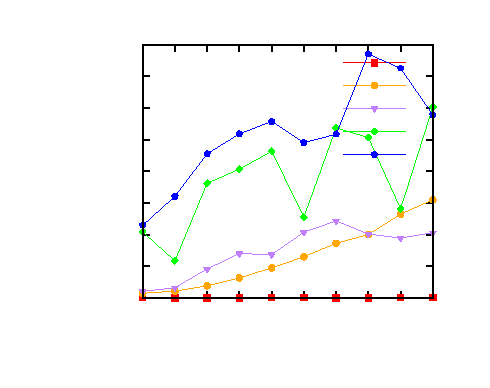
\includegraphics{bounds_epslatex/bounds_5_density_vs_time}}%
    \gplfronttext
  \end{picture}%
\endgroup

	% GNUPLOT: LaTeX picture with Postscript
\begingroup
  \makeatletter
  \providecommand\color[2][]{%
    \GenericError{(gnuplot) \space\space\space\@spaces}{%
      Package color not loaded in conjunction with
      terminal option `colourtext'%
    }{See the gnuplot documentation for explanation.%
    }{Either use 'blacktext' in gnuplot or load the package
      color.sty in LaTeX.}%
    \renewcommand\color[2][]{}%
  }%
  \providecommand\includegraphics[2][]{%
    \GenericError{(gnuplot) \space\space\space\@spaces}{%
      Package graphicx or graphics not loaded%
    }{See the gnuplot documentation for explanation.%
    }{The gnuplot epslatex terminal needs graphicx.sty or graphics.sty.}%
    \renewcommand\includegraphics[2][]{}%
  }%
  \providecommand\rotatebox[2]{#2}%
  \@ifundefined{ifGPcolor}{%
    \newif\ifGPcolor
    \GPcolorfalse
  }{}%
  \@ifundefined{ifGPblacktext}{%
    \newif\ifGPblacktext
    \GPblacktexttrue
  }{}%
  % define a \g@addto@macro without @ in the name:
  \let\gplgaddtomacro\g@addto@macro
  % define empty templates for all commands taking text:
  \gdef\gplbacktext{}%
  \gdef\gplfronttext{}%
  \makeatother
  \ifGPblacktext
    % no textcolor at all
    \def\colorrgb#1{}%
    \def\colorgray#1{}%
  \else
    % gray or color?
    \ifGPcolor
      \def\colorrgb#1{\color[rgb]{#1}}%
      \def\colorgray#1{\color[gray]{#1}}%
      \expandafter\def\csname LTw\endcsname{\color{white}}%
      \expandafter\def\csname LTb\endcsname{\color{black}}%
      \expandafter\def\csname LTa\endcsname{\color{black}}%
      \expandafter\def\csname LT0\endcsname{\color[rgb]{1,0,0}}%
      \expandafter\def\csname LT1\endcsname{\color[rgb]{0,1,0}}%
      \expandafter\def\csname LT2\endcsname{\color[rgb]{0,0,1}}%
      \expandafter\def\csname LT3\endcsname{\color[rgb]{1,0,1}}%
      \expandafter\def\csname LT4\endcsname{\color[rgb]{0,1,1}}%
      \expandafter\def\csname LT5\endcsname{\color[rgb]{1,1,0}}%
      \expandafter\def\csname LT6\endcsname{\color[rgb]{0,0,0}}%
      \expandafter\def\csname LT7\endcsname{\color[rgb]{1,0.3,0}}%
      \expandafter\def\csname LT8\endcsname{\color[rgb]{0.5,0.5,0.5}}%
    \else
      % gray
      \def\colorrgb#1{\color{black}}%
      \def\colorgray#1{\color[gray]{#1}}%
      \expandafter\def\csname LTw\endcsname{\color{white}}%
      \expandafter\def\csname LTb\endcsname{\color{black}}%
      \expandafter\def\csname LTa\endcsname{\color{black}}%
      \expandafter\def\csname LT0\endcsname{\color{black}}%
      \expandafter\def\csname LT1\endcsname{\color{black}}%
      \expandafter\def\csname LT2\endcsname{\color{black}}%
      \expandafter\def\csname LT3\endcsname{\color{black}}%
      \expandafter\def\csname LT4\endcsname{\color{black}}%
      \expandafter\def\csname LT5\endcsname{\color{black}}%
      \expandafter\def\csname LT6\endcsname{\color{black}}%
      \expandafter\def\csname LT7\endcsname{\color{black}}%
      \expandafter\def\csname LT8\endcsname{\color{black}}%
    \fi
  \fi
  \setlength{\unitlength}{0.0500bp}%
  \begin{picture}(4392.00,3400.00)%
    \gplgaddtomacro\gplbacktext{%
      \csname LTb\endcsname%
      \put(814,704){\makebox(0,0)[r]{\strut{} 0}}%
      \put(814,947){\makebox(0,0)[r]{\strut{} 2}}%
      \put(814,1190){\makebox(0,0)[r]{\strut{} 4}}%
      \put(814,1433){\makebox(0,0)[r]{\strut{} 6}}%
      \put(814,1676){\makebox(0,0)[r]{\strut{} 8}}%
      \put(814,1920){\makebox(0,0)[r]{\strut{} 10}}%
      \put(814,2163){\makebox(0,0)[r]{\strut{} 12}}%
      \put(814,2406){\makebox(0,0)[r]{\strut{} 14}}%
      \put(814,2649){\makebox(0,0)[r]{\strut{} 16}}%
      \put(814,2892){\makebox(0,0)[r]{\strut{} 18}}%
      \put(814,3135){\makebox(0,0)[r]{\strut{} 20}}%
      \put(946,484){\makebox(0,0){\strut{} 10}}%
      \put(1285,484){\makebox(0,0){\strut{} 20}}%
      \put(1624,484){\makebox(0,0){\strut{} 30}}%
      \put(1962,484){\makebox(0,0){\strut{} 40}}%
      \put(2301,484){\makebox(0,0){\strut{} 50}}%
      \put(2640,484){\makebox(0,0){\strut{} 60}}%
      \put(2979,484){\makebox(0,0){\strut{} 70}}%
      \put(3317,484){\makebox(0,0){\strut{} 80}}%
      \put(3656,484){\makebox(0,0){\strut{} 90}}%
      \put(3995,484){\makebox(0,0){\strut{} 100}}%
      \put(176,1919){\rotatebox{-270}{\makebox(0,0){\strut{}Tiempo de ejecuci\'on (ms)}}}%
      \put(2470,154){\makebox(0,0){\strut{}Porcentaje de clientes ($p$)}}%
    }%
    \gplgaddtomacro\gplfronttext{%
      \csname LTb\endcsname%
      \put(3008,2962){\makebox(0,0)[r]{\strut{}\texttt{dist\_x3}}}%
    }%
    \gplbacktext
    \put(0,0){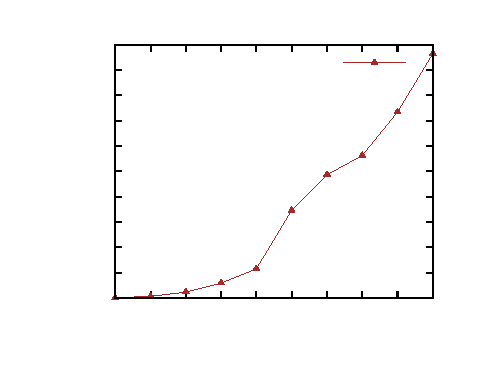
\includegraphics{bounds_epslatex/dist_x3_5_density_vs_time}}%
    \gplfronttext
  \end{picture}%
\endgroup

	\caption{Tiempos de ejecuci'on de las cotas para $n = 5$.}
	\label{fig:tiempos_5x5}
\end{figure}

\begin{figure}[h]
	% GNUPLOT: LaTeX picture with Postscript
\begingroup
  \makeatletter
  \providecommand\color[2][]{%
    \GenericError{(gnuplot) \space\space\space\@spaces}{%
      Package color not loaded in conjunction with
      terminal option `colourtext'%
    }{See the gnuplot documentation for explanation.%
    }{Either use 'blacktext' in gnuplot or load the package
      color.sty in LaTeX.}%
    \renewcommand\color[2][]{}%
  }%
  \providecommand\includegraphics[2][]{%
    \GenericError{(gnuplot) \space\space\space\@spaces}{%
      Package graphicx or graphics not loaded%
    }{See the gnuplot documentation for explanation.%
    }{The gnuplot epslatex terminal needs graphicx.sty or graphics.sty.}%
    \renewcommand\includegraphics[2][]{}%
  }%
  \providecommand\rotatebox[2]{#2}%
  \@ifundefined{ifGPcolor}{%
    \newif\ifGPcolor
    \GPcolorfalse
  }{}%
  \@ifundefined{ifGPblacktext}{%
    \newif\ifGPblacktext
    \GPblacktexttrue
  }{}%
  % define a \g@addto@macro without @ in the name:
  \let\gplgaddtomacro\g@addto@macro
  % define empty templates for all commands taking text:
  \gdef\gplbacktext{}%
  \gdef\gplfronttext{}%
  \makeatother
  \ifGPblacktext
    % no textcolor at all
    \def\colorrgb#1{}%
    \def\colorgray#1{}%
  \else
    % gray or color?
    \ifGPcolor
      \def\colorrgb#1{\color[rgb]{#1}}%
      \def\colorgray#1{\color[gray]{#1}}%
      \expandafter\def\csname LTw\endcsname{\color{white}}%
      \expandafter\def\csname LTb\endcsname{\color{black}}%
      \expandafter\def\csname LTa\endcsname{\color{black}}%
      \expandafter\def\csname LT0\endcsname{\color[rgb]{1,0,0}}%
      \expandafter\def\csname LT1\endcsname{\color[rgb]{0,1,0}}%
      \expandafter\def\csname LT2\endcsname{\color[rgb]{0,0,1}}%
      \expandafter\def\csname LT3\endcsname{\color[rgb]{1,0,1}}%
      \expandafter\def\csname LT4\endcsname{\color[rgb]{0,1,1}}%
      \expandafter\def\csname LT5\endcsname{\color[rgb]{1,1,0}}%
      \expandafter\def\csname LT6\endcsname{\color[rgb]{0,0,0}}%
      \expandafter\def\csname LT7\endcsname{\color[rgb]{1,0.3,0}}%
      \expandafter\def\csname LT8\endcsname{\color[rgb]{0.5,0.5,0.5}}%
    \else
      % gray
      \def\colorrgb#1{\color{black}}%
      \def\colorgray#1{\color[gray]{#1}}%
      \expandafter\def\csname LTw\endcsname{\color{white}}%
      \expandafter\def\csname LTb\endcsname{\color{black}}%
      \expandafter\def\csname LTa\endcsname{\color{black}}%
      \expandafter\def\csname LT0\endcsname{\color{black}}%
      \expandafter\def\csname LT1\endcsname{\color{black}}%
      \expandafter\def\csname LT2\endcsname{\color{black}}%
      \expandafter\def\csname LT3\endcsname{\color{black}}%
      \expandafter\def\csname LT4\endcsname{\color{black}}%
      \expandafter\def\csname LT5\endcsname{\color{black}}%
      \expandafter\def\csname LT6\endcsname{\color{black}}%
      \expandafter\def\csname LT7\endcsname{\color{black}}%
      \expandafter\def\csname LT8\endcsname{\color{black}}%
    \fi
  \fi
  \setlength{\unitlength}{0.0500bp}%
  \begin{picture}(4392.00,3400.00)%
    \gplgaddtomacro\gplbacktext{%
      \csname LTb\endcsname%
      \put(946,704){\makebox(0,0)[r]{\strut{} 0}}%
      \put(946,1051){\makebox(0,0)[r]{\strut{} 0.2}}%
      \put(946,1399){\makebox(0,0)[r]{\strut{} 0.4}}%
      \put(946,1746){\makebox(0,0)[r]{\strut{} 0.6}}%
      \put(946,2093){\makebox(0,0)[r]{\strut{} 0.8}}%
      \put(946,2440){\makebox(0,0)[r]{\strut{} 1}}%
      \put(946,2788){\makebox(0,0)[r]{\strut{} 1.2}}%
      \put(946,3135){\makebox(0,0)[r]{\strut{} 1.4}}%
      \put(1078,484){\makebox(0,0){\strut{} 10}}%
      \put(1402,484){\makebox(0,0){\strut{} 20}}%
      \put(1726,484){\makebox(0,0){\strut{} 30}}%
      \put(2050,484){\makebox(0,0){\strut{} 40}}%
      \put(2374,484){\makebox(0,0){\strut{} 50}}%
      \put(2699,484){\makebox(0,0){\strut{} 60}}%
      \put(3023,484){\makebox(0,0){\strut{} 70}}%
      \put(3347,484){\makebox(0,0){\strut{} 80}}%
      \put(3671,484){\makebox(0,0){\strut{} 90}}%
      \put(3995,484){\makebox(0,0){\strut{} 100}}%
      \put(176,1919){\rotatebox{-270}{\makebox(0,0){\strut{}Tiempo de ejecuci\'on (ms)}}}%
      \put(2536,154){\makebox(0,0){\strut{}Porcentaje de clientes ($p$)}}%
    }%
    \gplgaddtomacro\gplfronttext{%
      \csname LTb\endcsname%
      \put(3008,2962){\makebox(0,0)[r]{\strut{}\texttt{clients\_count}}}%
      \csname LTb\endcsname%
      \put(3008,2742){\makebox(0,0)[r]{\strut{}\texttt{dist\_x2}}}%
      \csname LTb\endcsname%
      \put(3008,2522){\makebox(0,0)[r]{\strut{}\texttt{mst}}}%
      \csname LTb\endcsname%
      \put(3008,2302){\makebox(0,0)[r]{\strut{}\texttt{vc}}}%
      \csname LTb\endcsname%
      \put(3008,2082){\makebox(0,0)[r]{\strut{}\texttt{vc\_mst}}}%
    }%
    \gplbacktext
    \put(0,0){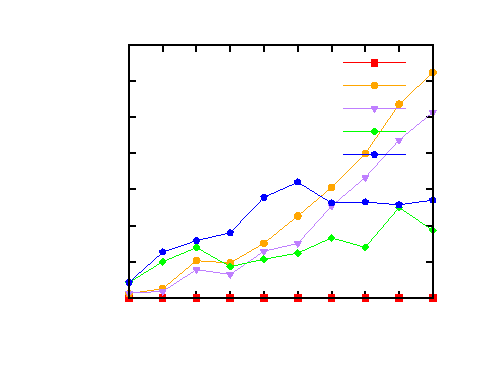
\includegraphics{bounds_epslatex/bounds_10_density_vs_time}}%
    \gplfronttext
  \end{picture}%
\endgroup

	% GNUPLOT: LaTeX picture with Postscript
\begingroup
  \makeatletter
  \providecommand\color[2][]{%
    \GenericError{(gnuplot) \space\space\space\@spaces}{%
      Package color not loaded in conjunction with
      terminal option `colourtext'%
    }{See the gnuplot documentation for explanation.%
    }{Either use 'blacktext' in gnuplot or load the package
      color.sty in LaTeX.}%
    \renewcommand\color[2][]{}%
  }%
  \providecommand\includegraphics[2][]{%
    \GenericError{(gnuplot) \space\space\space\@spaces}{%
      Package graphicx or graphics not loaded%
    }{See the gnuplot documentation for explanation.%
    }{The gnuplot epslatex terminal needs graphicx.sty or graphics.sty.}%
    \renewcommand\includegraphics[2][]{}%
  }%
  \providecommand\rotatebox[2]{#2}%
  \@ifundefined{ifGPcolor}{%
    \newif\ifGPcolor
    \GPcolorfalse
  }{}%
  \@ifundefined{ifGPblacktext}{%
    \newif\ifGPblacktext
    \GPblacktexttrue
  }{}%
  % define a \g@addto@macro without @ in the name:
  \let\gplgaddtomacro\g@addto@macro
  % define empty templates for all commands taking text:
  \gdef\gplbacktext{}%
  \gdef\gplfronttext{}%
  \makeatother
  \ifGPblacktext
    % no textcolor at all
    \def\colorrgb#1{}%
    \def\colorgray#1{}%
  \else
    % gray or color?
    \ifGPcolor
      \def\colorrgb#1{\color[rgb]{#1}}%
      \def\colorgray#1{\color[gray]{#1}}%
      \expandafter\def\csname LTw\endcsname{\color{white}}%
      \expandafter\def\csname LTb\endcsname{\color{black}}%
      \expandafter\def\csname LTa\endcsname{\color{black}}%
      \expandafter\def\csname LT0\endcsname{\color[rgb]{1,0,0}}%
      \expandafter\def\csname LT1\endcsname{\color[rgb]{0,1,0}}%
      \expandafter\def\csname LT2\endcsname{\color[rgb]{0,0,1}}%
      \expandafter\def\csname LT3\endcsname{\color[rgb]{1,0,1}}%
      \expandafter\def\csname LT4\endcsname{\color[rgb]{0,1,1}}%
      \expandafter\def\csname LT5\endcsname{\color[rgb]{1,1,0}}%
      \expandafter\def\csname LT6\endcsname{\color[rgb]{0,0,0}}%
      \expandafter\def\csname LT7\endcsname{\color[rgb]{1,0.3,0}}%
      \expandafter\def\csname LT8\endcsname{\color[rgb]{0.5,0.5,0.5}}%
    \else
      % gray
      \def\colorrgb#1{\color{black}}%
      \def\colorgray#1{\color[gray]{#1}}%
      \expandafter\def\csname LTw\endcsname{\color{white}}%
      \expandafter\def\csname LTb\endcsname{\color{black}}%
      \expandafter\def\csname LTa\endcsname{\color{black}}%
      \expandafter\def\csname LT0\endcsname{\color{black}}%
      \expandafter\def\csname LT1\endcsname{\color{black}}%
      \expandafter\def\csname LT2\endcsname{\color{black}}%
      \expandafter\def\csname LT3\endcsname{\color{black}}%
      \expandafter\def\csname LT4\endcsname{\color{black}}%
      \expandafter\def\csname LT5\endcsname{\color{black}}%
      \expandafter\def\csname LT6\endcsname{\color{black}}%
      \expandafter\def\csname LT7\endcsname{\color{black}}%
      \expandafter\def\csname LT8\endcsname{\color{black}}%
    \fi
  \fi
  \setlength{\unitlength}{0.0500bp}%
  \begin{picture}(4392.00,3400.00)%
    \gplgaddtomacro\gplbacktext{%
      \csname LTb\endcsname%
      \put(1078,704){\makebox(0,0)[r]{\strut{} 0}}%
      \put(1078,1051){\makebox(0,0)[r]{\strut{} 200}}%
      \put(1078,1399){\makebox(0,0)[r]{\strut{} 400}}%
      \put(1078,1746){\makebox(0,0)[r]{\strut{} 600}}%
      \put(1078,2093){\makebox(0,0)[r]{\strut{} 800}}%
      \put(1078,2440){\makebox(0,0)[r]{\strut{} 1000}}%
      \put(1078,2788){\makebox(0,0)[r]{\strut{} 1200}}%
      \put(1078,3135){\makebox(0,0)[r]{\strut{} 1400}}%
      \put(1210,484){\makebox(0,0){\strut{} 10}}%
      \put(1519,484){\makebox(0,0){\strut{} 20}}%
      \put(1829,484){\makebox(0,0){\strut{} 30}}%
      \put(2138,484){\makebox(0,0){\strut{} 40}}%
      \put(2448,484){\makebox(0,0){\strut{} 50}}%
      \put(2757,484){\makebox(0,0){\strut{} 60}}%
      \put(3067,484){\makebox(0,0){\strut{} 70}}%
      \put(3376,484){\makebox(0,0){\strut{} 80}}%
      \put(3686,484){\makebox(0,0){\strut{} 90}}%
      \put(3995,484){\makebox(0,0){\strut{} 100}}%
      \put(176,1919){\rotatebox{-270}{\makebox(0,0){\strut{}Tiempo de ejecuci\'on (ms)}}}%
      \put(2602,154){\makebox(0,0){\strut{}Porcentaje de clientes ($p$)}}%
    }%
    \gplgaddtomacro\gplfronttext{%
      \csname LTb\endcsname%
      \put(3008,2962){\makebox(0,0)[r]{\strut{}\texttt{dist\_x3}}}%
    }%
    \gplbacktext
    \put(0,0){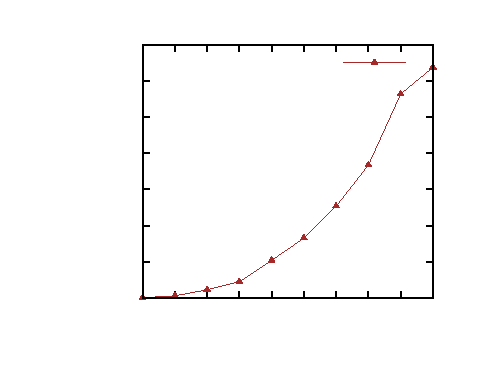
\includegraphics{bounds_epslatex/dist_x3_10_density_vs_time}}%
    \gplfronttext
  \end{picture}%
\endgroup

	\caption{Tiempos de ejecuci'on de las cotas para $n = 10$.}
	\label{fig:tiempos_10x10}
\end{figure}

\begin{figure}[h]
	% GNUPLOT: LaTeX picture with Postscript
\begingroup
  \makeatletter
  \providecommand\color[2][]{%
    \GenericError{(gnuplot) \space\space\space\@spaces}{%
      Package color not loaded in conjunction with
      terminal option `colourtext'%
    }{See the gnuplot documentation for explanation.%
    }{Either use 'blacktext' in gnuplot or load the package
      color.sty in LaTeX.}%
    \renewcommand\color[2][]{}%
  }%
  \providecommand\includegraphics[2][]{%
    \GenericError{(gnuplot) \space\space\space\@spaces}{%
      Package graphicx or graphics not loaded%
    }{See the gnuplot documentation for explanation.%
    }{The gnuplot epslatex terminal needs graphicx.sty or graphics.sty.}%
    \renewcommand\includegraphics[2][]{}%
  }%
  \providecommand\rotatebox[2]{#2}%
  \@ifundefined{ifGPcolor}{%
    \newif\ifGPcolor
    \GPcolorfalse
  }{}%
  \@ifundefined{ifGPblacktext}{%
    \newif\ifGPblacktext
    \GPblacktexttrue
  }{}%
  % define a \g@addto@macro without @ in the name:
  \let\gplgaddtomacro\g@addto@macro
  % define empty templates for all commands taking text:
  \gdef\gplbacktext{}%
  \gdef\gplfronttext{}%
  \makeatother
  \ifGPblacktext
    % no textcolor at all
    \def\colorrgb#1{}%
    \def\colorgray#1{}%
  \else
    % gray or color?
    \ifGPcolor
      \def\colorrgb#1{\color[rgb]{#1}}%
      \def\colorgray#1{\color[gray]{#1}}%
      \expandafter\def\csname LTw\endcsname{\color{white}}%
      \expandafter\def\csname LTb\endcsname{\color{black}}%
      \expandafter\def\csname LTa\endcsname{\color{black}}%
      \expandafter\def\csname LT0\endcsname{\color[rgb]{1,0,0}}%
      \expandafter\def\csname LT1\endcsname{\color[rgb]{0,1,0}}%
      \expandafter\def\csname LT2\endcsname{\color[rgb]{0,0,1}}%
      \expandafter\def\csname LT3\endcsname{\color[rgb]{1,0,1}}%
      \expandafter\def\csname LT4\endcsname{\color[rgb]{0,1,1}}%
      \expandafter\def\csname LT5\endcsname{\color[rgb]{1,1,0}}%
      \expandafter\def\csname LT6\endcsname{\color[rgb]{0,0,0}}%
      \expandafter\def\csname LT7\endcsname{\color[rgb]{1,0.3,0}}%
      \expandafter\def\csname LT8\endcsname{\color[rgb]{0.5,0.5,0.5}}%
    \else
      % gray
      \def\colorrgb#1{\color{black}}%
      \def\colorgray#1{\color[gray]{#1}}%
      \expandafter\def\csname LTw\endcsname{\color{white}}%
      \expandafter\def\csname LTb\endcsname{\color{black}}%
      \expandafter\def\csname LTa\endcsname{\color{black}}%
      \expandafter\def\csname LT0\endcsname{\color{black}}%
      \expandafter\def\csname LT1\endcsname{\color{black}}%
      \expandafter\def\csname LT2\endcsname{\color{black}}%
      \expandafter\def\csname LT3\endcsname{\color{black}}%
      \expandafter\def\csname LT4\endcsname{\color{black}}%
      \expandafter\def\csname LT5\endcsname{\color{black}}%
      \expandafter\def\csname LT6\endcsname{\color{black}}%
      \expandafter\def\csname LT7\endcsname{\color{black}}%
      \expandafter\def\csname LT8\endcsname{\color{black}}%
    \fi
  \fi
  \setlength{\unitlength}{0.0500bp}%
  \begin{picture}(4392.00,3400.00)%
    \gplgaddtomacro\gplbacktext{%
      \csname LTb\endcsname%
      \put(946,704){\makebox(0,0)[r]{\strut{} 0}}%
      \put(946,1051){\makebox(0,0)[r]{\strut{} 20}}%
      \put(946,1399){\makebox(0,0)[r]{\strut{} 40}}%
      \put(946,1746){\makebox(0,0)[r]{\strut{} 60}}%
      \put(946,2093){\makebox(0,0)[r]{\strut{} 80}}%
      \put(946,2440){\makebox(0,0)[r]{\strut{} 100}}%
      \put(946,2788){\makebox(0,0)[r]{\strut{} 120}}%
      \put(946,3135){\makebox(0,0)[r]{\strut{} 140}}%
      \put(1078,484){\makebox(0,0){\strut{} 10}}%
      \put(1402,484){\makebox(0,0){\strut{} 20}}%
      \put(1726,484){\makebox(0,0){\strut{} 30}}%
      \put(2050,484){\makebox(0,0){\strut{} 40}}%
      \put(2374,484){\makebox(0,0){\strut{} 50}}%
      \put(2699,484){\makebox(0,0){\strut{} 60}}%
      \put(3023,484){\makebox(0,0){\strut{} 70}}%
      \put(3347,484){\makebox(0,0){\strut{} 80}}%
      \put(3671,484){\makebox(0,0){\strut{} 90}}%
      \put(3995,484){\makebox(0,0){\strut{} 100}}%
      \put(176,1919){\rotatebox{-270}{\makebox(0,0){\strut{}Tiempo de ejecuci\'on (ms)}}}%
      \put(2536,154){\makebox(0,0){\strut{}Porcentaje de clientes ($p$)}}%
    }%
    \gplgaddtomacro\gplfronttext{%
      \csname LTb\endcsname%
      \put(3008,2962){\makebox(0,0)[r]{\strut{}\texttt{clients\_count}}}%
      \csname LTb\endcsname%
      \put(3008,2742){\makebox(0,0)[r]{\strut{}\texttt{dist\_x2}}}%
      \csname LTb\endcsname%
      \put(3008,2522){\makebox(0,0)[r]{\strut{}\texttt{mst}}}%
      \csname LTb\endcsname%
      \put(3008,2302){\makebox(0,0)[r]{\strut{}\texttt{vc}}}%
      \csname LTb\endcsname%
      \put(3008,2082){\makebox(0,0)[r]{\strut{}\texttt{vc\_mst}}}%
    }%
    \gplbacktext
    \put(0,0){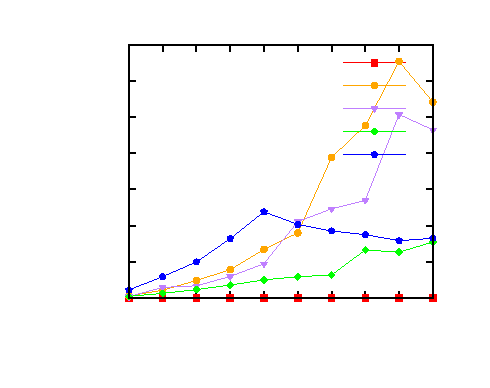
\includegraphics{bounds_epslatex/bounds_30_density_vs_time}}%
    \gplfronttext
  \end{picture}%
\endgroup

	% GNUPLOT: LaTeX picture with Postscript
\begingroup
  \makeatletter
  \providecommand\color[2][]{%
    \GenericError{(gnuplot) \space\space\space\@spaces}{%
      Package color not loaded in conjunction with
      terminal option `colourtext'%
    }{See the gnuplot documentation for explanation.%
    }{Either use 'blacktext' in gnuplot or load the package
      color.sty in LaTeX.}%
    \renewcommand\color[2][]{}%
  }%
  \providecommand\includegraphics[2][]{%
    \GenericError{(gnuplot) \space\space\space\@spaces}{%
      Package graphicx or graphics not loaded%
    }{See the gnuplot documentation for explanation.%
    }{The gnuplot epslatex terminal needs graphicx.sty or graphics.sty.}%
    \renewcommand\includegraphics[2][]{}%
  }%
  \providecommand\rotatebox[2]{#2}%
  \@ifundefined{ifGPcolor}{%
    \newif\ifGPcolor
    \GPcolorfalse
  }{}%
  \@ifundefined{ifGPblacktext}{%
    \newif\ifGPblacktext
    \GPblacktexttrue
  }{}%
  % define a \g@addto@macro without @ in the name:
  \let\gplgaddtomacro\g@addto@macro
  % define empty templates for all commands taking text:
  \gdef\gplbacktext{}%
  \gdef\gplfronttext{}%
  \makeatother
  \ifGPblacktext
    % no textcolor at all
    \def\colorrgb#1{}%
    \def\colorgray#1{}%
  \else
    % gray or color?
    \ifGPcolor
      \def\colorrgb#1{\color[rgb]{#1}}%
      \def\colorgray#1{\color[gray]{#1}}%
      \expandafter\def\csname LTw\endcsname{\color{white}}%
      \expandafter\def\csname LTb\endcsname{\color{black}}%
      \expandafter\def\csname LTa\endcsname{\color{black}}%
      \expandafter\def\csname LT0\endcsname{\color[rgb]{1,0,0}}%
      \expandafter\def\csname LT1\endcsname{\color[rgb]{0,1,0}}%
      \expandafter\def\csname LT2\endcsname{\color[rgb]{0,0,1}}%
      \expandafter\def\csname LT3\endcsname{\color[rgb]{1,0,1}}%
      \expandafter\def\csname LT4\endcsname{\color[rgb]{0,1,1}}%
      \expandafter\def\csname LT5\endcsname{\color[rgb]{1,1,0}}%
      \expandafter\def\csname LT6\endcsname{\color[rgb]{0,0,0}}%
      \expandafter\def\csname LT7\endcsname{\color[rgb]{1,0.3,0}}%
      \expandafter\def\csname LT8\endcsname{\color[rgb]{0.5,0.5,0.5}}%
    \else
      % gray
      \def\colorrgb#1{\color{black}}%
      \def\colorgray#1{\color[gray]{#1}}%
      \expandafter\def\csname LTw\endcsname{\color{white}}%
      \expandafter\def\csname LTb\endcsname{\color{black}}%
      \expandafter\def\csname LTa\endcsname{\color{black}}%
      \expandafter\def\csname LT0\endcsname{\color{black}}%
      \expandafter\def\csname LT1\endcsname{\color{black}}%
      \expandafter\def\csname LT2\endcsname{\color{black}}%
      \expandafter\def\csname LT3\endcsname{\color{black}}%
      \expandafter\def\csname LT4\endcsname{\color{black}}%
      \expandafter\def\csname LT5\endcsname{\color{black}}%
      \expandafter\def\csname LT6\endcsname{\color{black}}%
      \expandafter\def\csname LT7\endcsname{\color{black}}%
      \expandafter\def\csname LT8\endcsname{\color{black}}%
    \fi
  \fi
  \setlength{\unitlength}{0.0500bp}%
  \begin{picture}(4392.00,3400.00)%
    \gplgaddtomacro\gplbacktext{%
      \csname LTb\endcsname%
      \put(1474,704){\makebox(0,0)[r]{\strut{} 0}}%
      \put(1474,1051){\makebox(0,0)[r]{\strut{} 200000}}%
      \put(1474,1399){\makebox(0,0)[r]{\strut{} 400000}}%
      \put(1474,1746){\makebox(0,0)[r]{\strut{} 600000}}%
      \put(1474,2093){\makebox(0,0)[r]{\strut{} 800000}}%
      \put(1474,2440){\makebox(0,0)[r]{\strut{} 1e+06}}%
      \put(1474,2788){\makebox(0,0)[r]{\strut{} 1.2e+06}}%
      \put(1474,3135){\makebox(0,0)[r]{\strut{} 1.4e+06}}%
      \put(1606,484){\makebox(0,0){\strut{} 10}}%
      \put(1871,484){\makebox(0,0){\strut{} 20}}%
      \put(2137,484){\makebox(0,0){\strut{} 30}}%
      \put(2402,484){\makebox(0,0){\strut{} 40}}%
      \put(2668,484){\makebox(0,0){\strut{} 50}}%
      \put(2933,484){\makebox(0,0){\strut{} 60}}%
      \put(3199,484){\makebox(0,0){\strut{} 70}}%
      \put(3464,484){\makebox(0,0){\strut{} 80}}%
      \put(3730,484){\makebox(0,0){\strut{} 90}}%
      \put(3995,484){\makebox(0,0){\strut{} 100}}%
      \put(176,1919){\rotatebox{-270}{\makebox(0,0){\strut{}Tiempo de ejecuci\'on (ms)}}}%
      \put(2800,154){\makebox(0,0){\strut{}Porcentaje de clientes ($p$)}}%
    }%
    \gplgaddtomacro\gplfronttext{%
      \csname LTb\endcsname%
      \put(3008,2962){\makebox(0,0)[r]{\strut{}\texttt{dist\_x3}}}%
    }%
    \gplbacktext
    \put(0,0){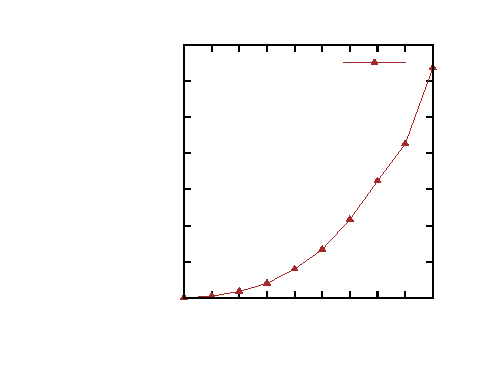
\includegraphics{bounds_epslatex/dist_x3_30_density_vs_time}}%
    \gplfronttext
  \end{picture}%
\endgroup

	\caption{Tiempos de ejecuci'on de las cotas para $n = 30$.}
	\label{fig:tiempos_30x30}
\end{figure}

\begin{figure}[h]
	\centering
	% GNUPLOT: LaTeX picture with Postscript
\begingroup
  \makeatletter
  \providecommand\color[2][]{%
    \GenericError{(gnuplot) \space\space\space\@spaces}{%
      Package color not loaded in conjunction with
      terminal option `colourtext'%
    }{See the gnuplot documentation for explanation.%
    }{Either use 'blacktext' in gnuplot or load the package
      color.sty in LaTeX.}%
    \renewcommand\color[2][]{}%
  }%
  \providecommand\includegraphics[2][]{%
    \GenericError{(gnuplot) \space\space\space\@spaces}{%
      Package graphicx or graphics not loaded%
    }{See the gnuplot documentation for explanation.%
    }{The gnuplot epslatex terminal needs graphicx.sty or graphics.sty.}%
    \renewcommand\includegraphics[2][]{}%
  }%
  \providecommand\rotatebox[2]{#2}%
  \@ifundefined{ifGPcolor}{%
    \newif\ifGPcolor
    \GPcolorfalse
  }{}%
  \@ifundefined{ifGPblacktext}{%
    \newif\ifGPblacktext
    \GPblacktexttrue
  }{}%
  % define a \g@addto@macro without @ in the name:
  \let\gplgaddtomacro\g@addto@macro
  % define empty templates for all commands taking text:
  \gdef\gplbacktext{}%
  \gdef\gplfronttext{}%
  \makeatother
  \ifGPblacktext
    % no textcolor at all
    \def\colorrgb#1{}%
    \def\colorgray#1{}%
  \else
    % gray or color?
    \ifGPcolor
      \def\colorrgb#1{\color[rgb]{#1}}%
      \def\colorgray#1{\color[gray]{#1}}%
      \expandafter\def\csname LTw\endcsname{\color{white}}%
      \expandafter\def\csname LTb\endcsname{\color{black}}%
      \expandafter\def\csname LTa\endcsname{\color{black}}%
      \expandafter\def\csname LT0\endcsname{\color[rgb]{1,0,0}}%
      \expandafter\def\csname LT1\endcsname{\color[rgb]{0,1,0}}%
      \expandafter\def\csname LT2\endcsname{\color[rgb]{0,0,1}}%
      \expandafter\def\csname LT3\endcsname{\color[rgb]{1,0,1}}%
      \expandafter\def\csname LT4\endcsname{\color[rgb]{0,1,1}}%
      \expandafter\def\csname LT5\endcsname{\color[rgb]{1,1,0}}%
      \expandafter\def\csname LT6\endcsname{\color[rgb]{0,0,0}}%
      \expandafter\def\csname LT7\endcsname{\color[rgb]{1,0.3,0}}%
      \expandafter\def\csname LT8\endcsname{\color[rgb]{0.5,0.5,0.5}}%
    \else
      % gray
      \def\colorrgb#1{\color{black}}%
      \def\colorgray#1{\color[gray]{#1}}%
      \expandafter\def\csname LTw\endcsname{\color{white}}%
      \expandafter\def\csname LTb\endcsname{\color{black}}%
      \expandafter\def\csname LTa\endcsname{\color{black}}%
      \expandafter\def\csname LT0\endcsname{\color{black}}%
      \expandafter\def\csname LT1\endcsname{\color{black}}%
      \expandafter\def\csname LT2\endcsname{\color{black}}%
      \expandafter\def\csname LT3\endcsname{\color{black}}%
      \expandafter\def\csname LT4\endcsname{\color{black}}%
      \expandafter\def\csname LT5\endcsname{\color{black}}%
      \expandafter\def\csname LT6\endcsname{\color{black}}%
      \expandafter\def\csname LT7\endcsname{\color{black}}%
      \expandafter\def\csname LT8\endcsname{\color{black}}%
    \fi
  \fi
  \setlength{\unitlength}{0.0500bp}%
  \begin{picture}(4392.00,3400.00)%
    \gplgaddtomacro\gplbacktext{%
      \csname LTb\endcsname%
      \put(946,704){\makebox(0,0)[r]{\strut{} 0}}%
      \put(946,974){\makebox(0,0)[r]{\strut{} 100}}%
      \put(946,1244){\makebox(0,0)[r]{\strut{} 200}}%
      \put(946,1514){\makebox(0,0)[r]{\strut{} 300}}%
      \put(946,1784){\makebox(0,0)[r]{\strut{} 400}}%
      \put(946,2055){\makebox(0,0)[r]{\strut{} 500}}%
      \put(946,2325){\makebox(0,0)[r]{\strut{} 600}}%
      \put(946,2595){\makebox(0,0)[r]{\strut{} 700}}%
      \put(946,2865){\makebox(0,0)[r]{\strut{} 800}}%
      \put(946,3135){\makebox(0,0)[r]{\strut{} 900}}%
      \put(1078,484){\makebox(0,0){\strut{} 10}}%
      \put(1402,484){\makebox(0,0){\strut{} 20}}%
      \put(1726,484){\makebox(0,0){\strut{} 30}}%
      \put(2050,484){\makebox(0,0){\strut{} 40}}%
      \put(2374,484){\makebox(0,0){\strut{} 50}}%
      \put(2699,484){\makebox(0,0){\strut{} 60}}%
      \put(3023,484){\makebox(0,0){\strut{} 70}}%
      \put(3347,484){\makebox(0,0){\strut{} 80}}%
      \put(3671,484){\makebox(0,0){\strut{} 90}}%
      \put(3995,484){\makebox(0,0){\strut{} 100}}%
      \put(176,1919){\rotatebox{-270}{\makebox(0,0){\strut{}Tiempo de ejecuci\'on (ms)}}}%
      \put(2536,154){\makebox(0,0){\strut{}Porcentaje de clientes ($p$)}}%
    }%
    \gplgaddtomacro\gplfronttext{%
      \csname LTb\endcsname%
      \put(3008,2962){\makebox(0,0)[r]{\strut{}\texttt{clients\_count}}}%
      \csname LTb\endcsname%
      \put(3008,2742){\makebox(0,0)[r]{\strut{}\texttt{dist\_x2}}}%
      \csname LTb\endcsname%
      \put(3008,2522){\makebox(0,0)[r]{\strut{}\texttt{mst}}}%
      \csname LTb\endcsname%
      \put(3008,2302){\makebox(0,0)[r]{\strut{}\texttt{vc}}}%
      \csname LTb\endcsname%
      \put(3008,2082){\makebox(0,0)[r]{\strut{}\texttt{vc\_mst}}}%
    }%
    \gplbacktext
    \put(0,0){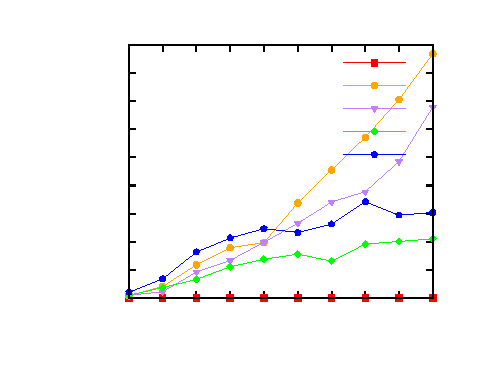
\includegraphics{bounds_epslatex/bounds_50_density_vs_time}}%
    \gplfronttext
  \end{picture}%
\endgroup

	\caption{Tiempos de ejecuci'on de las cotas para $n = 50$.}
	\label{fig:tiempos_50x50}
\end{figure}

\begin{figure}[h]
\begin{minipage}[t]{0.45\textwidth}
	\centering
	% GNUPLOT: LaTeX picture with Postscript
\begingroup
  \makeatletter
  \providecommand\color[2][]{%
    \GenericError{(gnuplot) \space\space\space\@spaces}{%
      Package color not loaded in conjunction with
      terminal option `colourtext'%
    }{See the gnuplot documentation for explanation.%
    }{Either use 'blacktext' in gnuplot or load the package
      color.sty in LaTeX.}%
    \renewcommand\color[2][]{}%
  }%
  \providecommand\includegraphics[2][]{%
    \GenericError{(gnuplot) \space\space\space\@spaces}{%
      Package graphicx or graphics not loaded%
    }{See the gnuplot documentation for explanation.%
    }{The gnuplot epslatex terminal needs graphicx.sty or graphics.sty.}%
    \renewcommand\includegraphics[2][]{}%
  }%
  \providecommand\rotatebox[2]{#2}%
  \@ifundefined{ifGPcolor}{%
    \newif\ifGPcolor
    \GPcolorfalse
  }{}%
  \@ifundefined{ifGPblacktext}{%
    \newif\ifGPblacktext
    \GPblacktexttrue
  }{}%
  % define a \g@addto@macro without @ in the name:
  \let\gplgaddtomacro\g@addto@macro
  % define empty templates for all commands taking text:
  \gdef\gplbacktext{}%
  \gdef\gplfronttext{}%
  \makeatother
  \ifGPblacktext
    % no textcolor at all
    \def\colorrgb#1{}%
    \def\colorgray#1{}%
  \else
    % gray or color?
    \ifGPcolor
      \def\colorrgb#1{\color[rgb]{#1}}%
      \def\colorgray#1{\color[gray]{#1}}%
      \expandafter\def\csname LTw\endcsname{\color{white}}%
      \expandafter\def\csname LTb\endcsname{\color{black}}%
      \expandafter\def\csname LTa\endcsname{\color{black}}%
      \expandafter\def\csname LT0\endcsname{\color[rgb]{1,0,0}}%
      \expandafter\def\csname LT1\endcsname{\color[rgb]{0,1,0}}%
      \expandafter\def\csname LT2\endcsname{\color[rgb]{0,0,1}}%
      \expandafter\def\csname LT3\endcsname{\color[rgb]{1,0,1}}%
      \expandafter\def\csname LT4\endcsname{\color[rgb]{0,1,1}}%
      \expandafter\def\csname LT5\endcsname{\color[rgb]{1,1,0}}%
      \expandafter\def\csname LT6\endcsname{\color[rgb]{0,0,0}}%
      \expandafter\def\csname LT7\endcsname{\color[rgb]{1,0.3,0}}%
      \expandafter\def\csname LT8\endcsname{\color[rgb]{0.5,0.5,0.5}}%
    \else
      % gray
      \def\colorrgb#1{\color{black}}%
      \def\colorgray#1{\color[gray]{#1}}%
      \expandafter\def\csname LTw\endcsname{\color{white}}%
      \expandafter\def\csname LTb\endcsname{\color{black}}%
      \expandafter\def\csname LTa\endcsname{\color{black}}%
      \expandafter\def\csname LT0\endcsname{\color{black}}%
      \expandafter\def\csname LT1\endcsname{\color{black}}%
      \expandafter\def\csname LT2\endcsname{\color{black}}%
      \expandafter\def\csname LT3\endcsname{\color{black}}%
      \expandafter\def\csname LT4\endcsname{\color{black}}%
      \expandafter\def\csname LT5\endcsname{\color{black}}%
      \expandafter\def\csname LT6\endcsname{\color{black}}%
      \expandafter\def\csname LT7\endcsname{\color{black}}%
      \expandafter\def\csname LT8\endcsname{\color{black}}%
    \fi
  \fi
  \setlength{\unitlength}{0.0500bp}%
  \begin{picture}(4392.00,3400.00)%
    \gplgaddtomacro\gplbacktext{%
      \csname LTb\endcsname%
      \put(814,704){\makebox(0,0)[r]{\strut{} 0}}%
      \put(814,1109){\makebox(0,0)[r]{\strut{} 2}}%
      \put(814,1514){\makebox(0,0)[r]{\strut{} 4}}%
      \put(814,1920){\makebox(0,0)[r]{\strut{} 6}}%
      \put(814,2325){\makebox(0,0)[r]{\strut{} 8}}%
      \put(814,2730){\makebox(0,0)[r]{\strut{} 10}}%
      \put(814,3135){\makebox(0,0)[r]{\strut{} 12}}%
      \put(946,484){\makebox(0,0){\strut{} 10}}%
      \put(1285,484){\makebox(0,0){\strut{} 20}}%
      \put(1624,484){\makebox(0,0){\strut{} 30}}%
      \put(1962,484){\makebox(0,0){\strut{} 40}}%
      \put(2301,484){\makebox(0,0){\strut{} 50}}%
      \put(2640,484){\makebox(0,0){\strut{} 60}}%
      \put(2979,484){\makebox(0,0){\strut{} 70}}%
      \put(3317,484){\makebox(0,0){\strut{} 80}}%
      \put(3656,484){\makebox(0,0){\strut{} 90}}%
      \put(3995,484){\makebox(0,0){\strut{} 100}}%
      \put(176,1919){\rotatebox{-270}{\makebox(0,0){\strut{}Valor de la funci\'on}}}%
      \put(2470,154){\makebox(0,0){\strut{}Porcentaje de clientes ($p$)}}%
    }%
    \gplgaddtomacro\gplfronttext{%
      \csname LTb\endcsname%
      \put(3008,2962){\makebox(0,0)[r]{\strut{}\texttt{clients\_count}}}%
      \csname LTb\endcsname%
      \put(3008,2742){\makebox(0,0)[r]{\strut{}\texttt{dist\_x2}}}%
      \csname LTb\endcsname%
      \put(3008,2522){\makebox(0,0)[r]{\strut{}\texttt{dist\_x3}}}%
      \csname LTb\endcsname%
      \put(3008,2302){\makebox(0,0)[r]{\strut{}\texttt{mst}}}%
      \csname LTb\endcsname%
      \put(3008,2082){\makebox(0,0)[r]{\strut{}\texttt{vc}}}%
      \csname LTb\endcsname%
      \put(3008,1862){\makebox(0,0)[r]{\strut{}\texttt{vc\_mst}}}%
    }%
    \gplbacktext
    \put(0,0){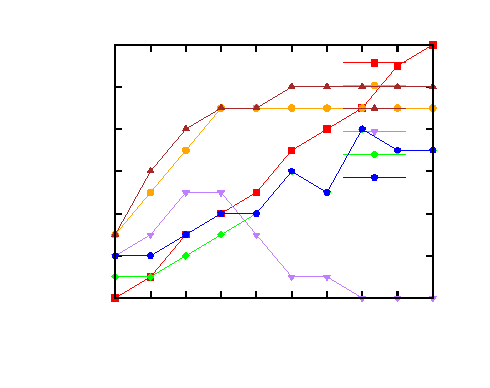
\includegraphics{bounds_epslatex/bounds_5_density_vs_value}}%
    \gplfronttext
  \end{picture}%
\endgroup

	\setcaptionwidth{5cm}
	\caption{Valores de las cotas para $n = 5$.}
	\label{fig:valores_5x5}
\end{minipage}%
\hfill%
\begin{minipage}[t]{0.45\textwidth}
	\centering
	% GNUPLOT: LaTeX picture with Postscript
\begingroup
  \makeatletter
  \providecommand\color[2][]{%
    \GenericError{(gnuplot) \space\space\space\@spaces}{%
      Package color not loaded in conjunction with
      terminal option `colourtext'%
    }{See the gnuplot documentation for explanation.%
    }{Either use 'blacktext' in gnuplot or load the package
      color.sty in LaTeX.}%
    \renewcommand\color[2][]{}%
  }%
  \providecommand\includegraphics[2][]{%
    \GenericError{(gnuplot) \space\space\space\@spaces}{%
      Package graphicx or graphics not loaded%
    }{See the gnuplot documentation for explanation.%
    }{The gnuplot epslatex terminal needs graphicx.sty or graphics.sty.}%
    \renewcommand\includegraphics[2][]{}%
  }%
  \providecommand\rotatebox[2]{#2}%
  \@ifundefined{ifGPcolor}{%
    \newif\ifGPcolor
    \GPcolorfalse
  }{}%
  \@ifundefined{ifGPblacktext}{%
    \newif\ifGPblacktext
    \GPblacktexttrue
  }{}%
  % define a \g@addto@macro without @ in the name:
  \let\gplgaddtomacro\g@addto@macro
  % define empty templates for all commands taking text:
  \gdef\gplbacktext{}%
  \gdef\gplfronttext{}%
  \makeatother
  \ifGPblacktext
    % no textcolor at all
    \def\colorrgb#1{}%
    \def\colorgray#1{}%
  \else
    % gray or color?
    \ifGPcolor
      \def\colorrgb#1{\color[rgb]{#1}}%
      \def\colorgray#1{\color[gray]{#1}}%
      \expandafter\def\csname LTw\endcsname{\color{white}}%
      \expandafter\def\csname LTb\endcsname{\color{black}}%
      \expandafter\def\csname LTa\endcsname{\color{black}}%
      \expandafter\def\csname LT0\endcsname{\color[rgb]{1,0,0}}%
      \expandafter\def\csname LT1\endcsname{\color[rgb]{0,1,0}}%
      \expandafter\def\csname LT2\endcsname{\color[rgb]{0,0,1}}%
      \expandafter\def\csname LT3\endcsname{\color[rgb]{1,0,1}}%
      \expandafter\def\csname LT4\endcsname{\color[rgb]{0,1,1}}%
      \expandafter\def\csname LT5\endcsname{\color[rgb]{1,1,0}}%
      \expandafter\def\csname LT6\endcsname{\color[rgb]{0,0,0}}%
      \expandafter\def\csname LT7\endcsname{\color[rgb]{1,0.3,0}}%
      \expandafter\def\csname LT8\endcsname{\color[rgb]{0.5,0.5,0.5}}%
    \else
      % gray
      \def\colorrgb#1{\color{black}}%
      \def\colorgray#1{\color[gray]{#1}}%
      \expandafter\def\csname LTw\endcsname{\color{white}}%
      \expandafter\def\csname LTb\endcsname{\color{black}}%
      \expandafter\def\csname LTa\endcsname{\color{black}}%
      \expandafter\def\csname LT0\endcsname{\color{black}}%
      \expandafter\def\csname LT1\endcsname{\color{black}}%
      \expandafter\def\csname LT2\endcsname{\color{black}}%
      \expandafter\def\csname LT3\endcsname{\color{black}}%
      \expandafter\def\csname LT4\endcsname{\color{black}}%
      \expandafter\def\csname LT5\endcsname{\color{black}}%
      \expandafter\def\csname LT6\endcsname{\color{black}}%
      \expandafter\def\csname LT7\endcsname{\color{black}}%
      \expandafter\def\csname LT8\endcsname{\color{black}}%
    \fi
  \fi
  \setlength{\unitlength}{0.0500bp}%
  \begin{picture}(4392.00,3400.00)%
    \gplgaddtomacro\gplbacktext{%
      \csname LTb\endcsname%
      \put(814,704){\makebox(0,0)[r]{\strut{} 0}}%
      \put(814,1109){\makebox(0,0)[r]{\strut{} 10}}%
      \put(814,1514){\makebox(0,0)[r]{\strut{} 20}}%
      \put(814,1920){\makebox(0,0)[r]{\strut{} 30}}%
      \put(814,2325){\makebox(0,0)[r]{\strut{} 40}}%
      \put(814,2730){\makebox(0,0)[r]{\strut{} 50}}%
      \put(814,3135){\makebox(0,0)[r]{\strut{} 60}}%
      \put(946,484){\makebox(0,0){\strut{} 10}}%
      \put(1285,484){\makebox(0,0){\strut{} 20}}%
      \put(1624,484){\makebox(0,0){\strut{} 30}}%
      \put(1962,484){\makebox(0,0){\strut{} 40}}%
      \put(2301,484){\makebox(0,0){\strut{} 50}}%
      \put(2640,484){\makebox(0,0){\strut{} 60}}%
      \put(2979,484){\makebox(0,0){\strut{} 70}}%
      \put(3317,484){\makebox(0,0){\strut{} 80}}%
      \put(3656,484){\makebox(0,0){\strut{} 90}}%
      \put(3995,484){\makebox(0,0){\strut{} 100}}%
      \put(176,1919){\rotatebox{-270}{\makebox(0,0){\strut{}Valor de la funci\'on}}}%
      \put(2470,154){\makebox(0,0){\strut{}Porcentaje de clientes ($p$)}}%
    }%
    \gplgaddtomacro\gplfronttext{%
      \csname LTb\endcsname%
      \put(3008,2962){\makebox(0,0)[r]{\strut{}\texttt{clients\_count}}}%
      \csname LTb\endcsname%
      \put(3008,2742){\makebox(0,0)[r]{\strut{}\texttt{dist\_x2}}}%
      \csname LTb\endcsname%
      \put(3008,2522){\makebox(0,0)[r]{\strut{}\texttt{dist\_x3}}}%
      \csname LTb\endcsname%
      \put(3008,2302){\makebox(0,0)[r]{\strut{}\texttt{mst}}}%
      \csname LTb\endcsname%
      \put(3008,2082){\makebox(0,0)[r]{\strut{}\texttt{vc}}}%
      \csname LTb\endcsname%
      \put(3008,1862){\makebox(0,0)[r]{\strut{}\texttt{vc\_mst}}}%
    }%
    \gplbacktext
    \put(0,0){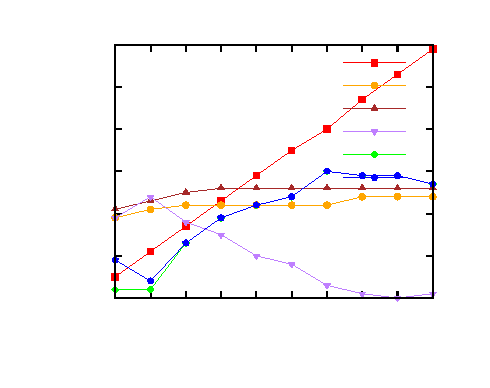
\includegraphics{bounds_epslatex/bounds_10_density_vs_value}}%
    \gplfronttext
  \end{picture}%
\endgroup

	\setcaptionwidth{5cm}
    \caption{Valores de las cotas para $n = 10$.}
	\label{fig:valores_10x10}
\end{minipage}

\begin{minipage}[t]{0.45\textwidth}
	\centering
	% GNUPLOT: LaTeX picture with Postscript
\begingroup
  \makeatletter
  \providecommand\color[2][]{%
    \GenericError{(gnuplot) \space\space\space\@spaces}{%
      Package color not loaded in conjunction with
      terminal option `colourtext'%
    }{See the gnuplot documentation for explanation.%
    }{Either use 'blacktext' in gnuplot or load the package
      color.sty in LaTeX.}%
    \renewcommand\color[2][]{}%
  }%
  \providecommand\includegraphics[2][]{%
    \GenericError{(gnuplot) \space\space\space\@spaces}{%
      Package graphicx or graphics not loaded%
    }{See the gnuplot documentation for explanation.%
    }{The gnuplot epslatex terminal needs graphicx.sty or graphics.sty.}%
    \renewcommand\includegraphics[2][]{}%
  }%
  \providecommand\rotatebox[2]{#2}%
  \@ifundefined{ifGPcolor}{%
    \newif\ifGPcolor
    \GPcolorfalse
  }{}%
  \@ifundefined{ifGPblacktext}{%
    \newif\ifGPblacktext
    \GPblacktexttrue
  }{}%
  % define a \g@addto@macro without @ in the name:
  \let\gplgaddtomacro\g@addto@macro
  % define empty templates for all commands taking text:
  \gdef\gplbacktext{}%
  \gdef\gplfronttext{}%
  \makeatother
  \ifGPblacktext
    % no textcolor at all
    \def\colorrgb#1{}%
    \def\colorgray#1{}%
  \else
    % gray or color?
    \ifGPcolor
      \def\colorrgb#1{\color[rgb]{#1}}%
      \def\colorgray#1{\color[gray]{#1}}%
      \expandafter\def\csname LTw\endcsname{\color{white}}%
      \expandafter\def\csname LTb\endcsname{\color{black}}%
      \expandafter\def\csname LTa\endcsname{\color{black}}%
      \expandafter\def\csname LT0\endcsname{\color[rgb]{1,0,0}}%
      \expandafter\def\csname LT1\endcsname{\color[rgb]{0,1,0}}%
      \expandafter\def\csname LT2\endcsname{\color[rgb]{0,0,1}}%
      \expandafter\def\csname LT3\endcsname{\color[rgb]{1,0,1}}%
      \expandafter\def\csname LT4\endcsname{\color[rgb]{0,1,1}}%
      \expandafter\def\csname LT5\endcsname{\color[rgb]{1,1,0}}%
      \expandafter\def\csname LT6\endcsname{\color[rgb]{0,0,0}}%
      \expandafter\def\csname LT7\endcsname{\color[rgb]{1,0.3,0}}%
      \expandafter\def\csname LT8\endcsname{\color[rgb]{0.5,0.5,0.5}}%
    \else
      % gray
      \def\colorrgb#1{\color{black}}%
      \def\colorgray#1{\color[gray]{#1}}%
      \expandafter\def\csname LTw\endcsname{\color{white}}%
      \expandafter\def\csname LTb\endcsname{\color{black}}%
      \expandafter\def\csname LTa\endcsname{\color{black}}%
      \expandafter\def\csname LT0\endcsname{\color{black}}%
      \expandafter\def\csname LT1\endcsname{\color{black}}%
      \expandafter\def\csname LT2\endcsname{\color{black}}%
      \expandafter\def\csname LT3\endcsname{\color{black}}%
      \expandafter\def\csname LT4\endcsname{\color{black}}%
      \expandafter\def\csname LT5\endcsname{\color{black}}%
      \expandafter\def\csname LT6\endcsname{\color{black}}%
      \expandafter\def\csname LT7\endcsname{\color{black}}%
      \expandafter\def\csname LT8\endcsname{\color{black}}%
    \fi
  \fi
  \setlength{\unitlength}{0.0500bp}%
  \begin{picture}(4392.00,3400.00)%
    \gplgaddtomacro\gplbacktext{%
      \csname LTb\endcsname%
      \put(946,704){\makebox(0,0)[r]{\strut{} 0}}%
      \put(946,1109){\makebox(0,0)[r]{\strut{} 100}}%
      \put(946,1514){\makebox(0,0)[r]{\strut{} 200}}%
      \put(946,1920){\makebox(0,0)[r]{\strut{} 300}}%
      \put(946,2325){\makebox(0,0)[r]{\strut{} 400}}%
      \put(946,2730){\makebox(0,0)[r]{\strut{} 500}}%
      \put(946,3135){\makebox(0,0)[r]{\strut{} 600}}%
      \put(1078,484){\makebox(0,0){\strut{} 10}}%
      \put(1402,484){\makebox(0,0){\strut{} 20}}%
      \put(1726,484){\makebox(0,0){\strut{} 30}}%
      \put(2050,484){\makebox(0,0){\strut{} 40}}%
      \put(2374,484){\makebox(0,0){\strut{} 50}}%
      \put(2699,484){\makebox(0,0){\strut{} 60}}%
      \put(3023,484){\makebox(0,0){\strut{} 70}}%
      \put(3347,484){\makebox(0,0){\strut{} 80}}%
      \put(3671,484){\makebox(0,0){\strut{} 90}}%
      \put(3995,484){\makebox(0,0){\strut{} 100}}%
      \put(176,1919){\rotatebox{-270}{\makebox(0,0){\strut{}Valor de la funci\'on}}}%
      \put(2536,154){\makebox(0,0){\strut{}Porcentaje de clientes ($p$)}}%
    }%
    \gplgaddtomacro\gplfronttext{%
      \csname LTb\endcsname%
      \put(3008,2962){\makebox(0,0)[r]{\strut{}\texttt{clients\_count}}}%
      \csname LTb\endcsname%
      \put(3008,2742){\makebox(0,0)[r]{\strut{}\texttt{dist\_x2}}}%
      \csname LTb\endcsname%
      \put(3008,2522){\makebox(0,0)[r]{\strut{}\texttt{dist\_x3}}}%
      \csname LTb\endcsname%
      \put(3008,2302){\makebox(0,0)[r]{\strut{}\texttt{mst}}}%
      \csname LTb\endcsname%
      \put(3008,2082){\makebox(0,0)[r]{\strut{}\texttt{vc}}}%
      \csname LTb\endcsname%
      \put(3008,1862){\makebox(0,0)[r]{\strut{}\texttt{vc\_mst}}}%
    }%
    \gplbacktext
    \put(0,0){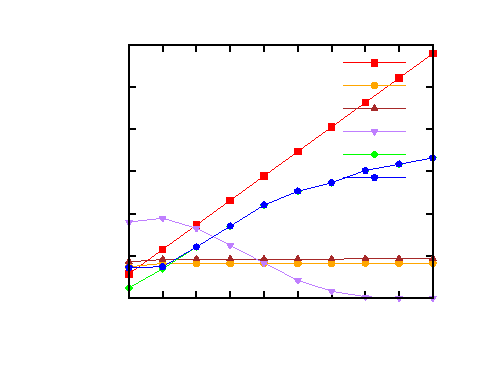
\includegraphics{bounds_epslatex/bounds_30_density_vs_value}}%
    \gplfronttext
  \end{picture}%
\endgroup

	\setcaptionwidth{5cm}
	\caption{Valores de las cotas para $n = 30$.}
	\label{fig:valores_30x30}
\end{minipage}%
\hfill%
\begin{minipage}[t]{0.45\textwidth}
	\centering
	% GNUPLOT: LaTeX picture with Postscript
\begingroup
  \makeatletter
  \providecommand\color[2][]{%
    \GenericError{(gnuplot) \space\space\space\@spaces}{%
      Package color not loaded in conjunction with
      terminal option `colourtext'%
    }{See the gnuplot documentation for explanation.%
    }{Either use 'blacktext' in gnuplot or load the package
      color.sty in LaTeX.}%
    \renewcommand\color[2][]{}%
  }%
  \providecommand\includegraphics[2][]{%
    \GenericError{(gnuplot) \space\space\space\@spaces}{%
      Package graphicx or graphics not loaded%
    }{See the gnuplot documentation for explanation.%
    }{The gnuplot epslatex terminal needs graphicx.sty or graphics.sty.}%
    \renewcommand\includegraphics[2][]{}%
  }%
  \providecommand\rotatebox[2]{#2}%
  \@ifundefined{ifGPcolor}{%
    \newif\ifGPcolor
    \GPcolorfalse
  }{}%
  \@ifundefined{ifGPblacktext}{%
    \newif\ifGPblacktext
    \GPblacktexttrue
  }{}%
  % define a \g@addto@macro without @ in the name:
  \let\gplgaddtomacro\g@addto@macro
  % define empty templates for all commands taking text:
  \gdef\gplbacktext{}%
  \gdef\gplfronttext{}%
  \makeatother
  \ifGPblacktext
    % no textcolor at all
    \def\colorrgb#1{}%
    \def\colorgray#1{}%
  \else
    % gray or color?
    \ifGPcolor
      \def\colorrgb#1{\color[rgb]{#1}}%
      \def\colorgray#1{\color[gray]{#1}}%
      \expandafter\def\csname LTw\endcsname{\color{white}}%
      \expandafter\def\csname LTb\endcsname{\color{black}}%
      \expandafter\def\csname LTa\endcsname{\color{black}}%
      \expandafter\def\csname LT0\endcsname{\color[rgb]{1,0,0}}%
      \expandafter\def\csname LT1\endcsname{\color[rgb]{0,1,0}}%
      \expandafter\def\csname LT2\endcsname{\color[rgb]{0,0,1}}%
      \expandafter\def\csname LT3\endcsname{\color[rgb]{1,0,1}}%
      \expandafter\def\csname LT4\endcsname{\color[rgb]{0,1,1}}%
      \expandafter\def\csname LT5\endcsname{\color[rgb]{1,1,0}}%
      \expandafter\def\csname LT6\endcsname{\color[rgb]{0,0,0}}%
      \expandafter\def\csname LT7\endcsname{\color[rgb]{1,0.3,0}}%
      \expandafter\def\csname LT8\endcsname{\color[rgb]{0.5,0.5,0.5}}%
    \else
      % gray
      \def\colorrgb#1{\color{black}}%
      \def\colorgray#1{\color[gray]{#1}}%
      \expandafter\def\csname LTw\endcsname{\color{white}}%
      \expandafter\def\csname LTb\endcsname{\color{black}}%
      \expandafter\def\csname LTa\endcsname{\color{black}}%
      \expandafter\def\csname LT0\endcsname{\color{black}}%
      \expandafter\def\csname LT1\endcsname{\color{black}}%
      \expandafter\def\csname LT2\endcsname{\color{black}}%
      \expandafter\def\csname LT3\endcsname{\color{black}}%
      \expandafter\def\csname LT4\endcsname{\color{black}}%
      \expandafter\def\csname LT5\endcsname{\color{black}}%
      \expandafter\def\csname LT6\endcsname{\color{black}}%
      \expandafter\def\csname LT7\endcsname{\color{black}}%
      \expandafter\def\csname LT8\endcsname{\color{black}}%
    \fi
  \fi
  \setlength{\unitlength}{0.0500bp}%
  \begin{picture}(4392.00,3400.00)%
    \gplgaddtomacro\gplbacktext{%
      \csname LTb\endcsname%
      \put(1078,704){\makebox(0,0)[r]{\strut{} 0}}%
      \put(1078,974){\makebox(0,0)[r]{\strut{} 200}}%
      \put(1078,1244){\makebox(0,0)[r]{\strut{} 400}}%
      \put(1078,1514){\makebox(0,0)[r]{\strut{} 600}}%
      \put(1078,1784){\makebox(0,0)[r]{\strut{} 800}}%
      \put(1078,2055){\makebox(0,0)[r]{\strut{} 1000}}%
      \put(1078,2325){\makebox(0,0)[r]{\strut{} 1200}}%
      \put(1078,2595){\makebox(0,0)[r]{\strut{} 1400}}%
      \put(1078,2865){\makebox(0,0)[r]{\strut{} 1600}}%
      \put(1078,3135){\makebox(0,0)[r]{\strut{} 1800}}%
      \put(1210,484){\makebox(0,0){\strut{} 10}}%
      \put(1519,484){\makebox(0,0){\strut{} 20}}%
      \put(1829,484){\makebox(0,0){\strut{} 30}}%
      \put(2138,484){\makebox(0,0){\strut{} 40}}%
      \put(2448,484){\makebox(0,0){\strut{} 50}}%
      \put(2757,484){\makebox(0,0){\strut{} 60}}%
      \put(3067,484){\makebox(0,0){\strut{} 70}}%
      \put(3376,484){\makebox(0,0){\strut{} 80}}%
      \put(3686,484){\makebox(0,0){\strut{} 90}}%
      \put(3995,484){\makebox(0,0){\strut{} 100}}%
      \put(176,1919){\rotatebox{-270}{\makebox(0,0){\strut{}Valor de la funci\'on}}}%
      \put(2602,154){\makebox(0,0){\strut{}Porcentaje de clientes ($p$)}}%
    }%
    \gplgaddtomacro\gplfronttext{%
      \csname LTb\endcsname%
      \put(3008,2962){\makebox(0,0)[r]{\strut{}\texttt{clients\_count}}}%
      \csname LTb\endcsname%
      \put(3008,2742){\makebox(0,0)[r]{\strut{}\texttt{dist\_x2}}}%
      \csname LTb\endcsname%
      \put(3008,2522){\makebox(0,0)[r]{\strut{}\texttt{mst}}}%
      \csname LTb\endcsname%
      \put(3008,2302){\makebox(0,0)[r]{\strut{}\texttt{vc}}}%
      \csname LTb\endcsname%
      \put(3008,2082){\makebox(0,0)[r]{\strut{}\texttt{vc\_mst}}}%
    }%
    \gplbacktext
    \put(0,0){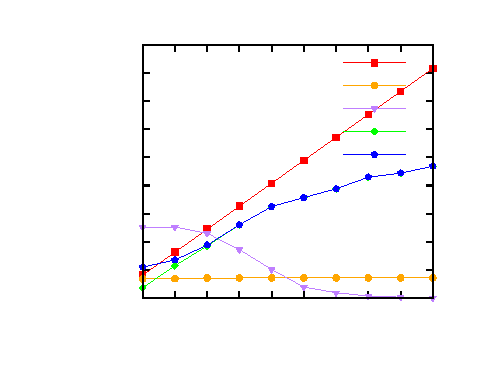
\includegraphics{bounds_epslatex/bounds_50_density_vs_value}}%
    \gplfronttext
  \end{picture}%
\endgroup

	\setcaptionwidth{5cm}
    \caption{Valores de las cotas para $n = 50$.}
	\label{fig:valores_50x50}
\end{minipage}
\end{figure}

\clearpage

La primera conclusi'on que se puede sacar es que las mediciones (tanto de tiempo de ejecuci'on como de valor de las cotas) convergen a medida que $n$ crece, lo cual se observa en la tendencia de los resultados para $n = 10, 30$ y  $50$. Lo segundo que se observa es que los resultados para $n = 5$ no siguen el patr'on general, lo cual es razonable, debido a que las instancias de ese tama\~no son demasiado chicas. En lo que sigue, s'olo analizamos los resultados para $n = 10, 30$ y $50$.

En todos los casos, la cota m'as costosa es \texttt{dist\_x3}, que insume tres o m'as 'ordenes de magnitud m'as de tiempo que el resto de las cotas. Dejamos de lado esta cota para analizar y comparar el resto. Se puede ver todas las cotas mantienen, aproximado, el mismo orden relativo a medida que $p$ crece, excepto por \texttt{vc\_mst}, que comienza siendo la m'as costosa pero es superada por \texttt{dist\_x2} y \texttt{mst}. La \autoref{ta:rankings_tiempos} muestra el ranking aproximado de cotas, por tiempos de ejecuci'on, seg'un indica la tendencia general. Para construir este ranking particionamos la escala de porcentajes en tres intervalos, $[10, 30)$, $[30, 50)$ y $[50, 100]$, elegidos en base a las variaciones de costo y efectividad que observamos en los gr'aficos. En cada intervalo, el ranking de cada cota est'a dado por una estimaci'on del 'area debajo de su curva, de la \autoref{fig:tiempos_30x30}.

\begin{table}[h]
\begin{center}
\begin{tabular}{|c|c|c|c|c|}
\hline
\# & $p \in [10, 30)$ & $p \in [30, 50)$ & $p \in [50, 100]$\\
\hline
1 & \texttt{dist\_x3} & \texttt{dist\_x3} & \texttt{dist\_x3}\\
2 & \texttt{vc\_mst} & \texttt{vc\_mst} & \texttt{dist\_x2} (+1)\\
3 & \texttt{dist\_x2} & \texttt{dist\_x2} & \texttt{mst} (+1)\\
4 & \texttt{mst} & \texttt{mst} & \texttt{vc\_mst} (-2)\\
5 & \texttt{vc} & \texttt{vc} & \texttt{vc}\\
6 & \texttt{clients\_count} & \texttt{clients\_count} & \texttt{clients\_count}\\
\hline
\end{tabular}
\end{center}
\caption{Ranking aproximado de cotas, por tiempo de ejecuci'on.}
\label{ta:rankings_tiempos}
\end{table}

Elaboramos el mismo ranking aproximado para la efectividad de las cotas, que se muestra en la \autoref{ta:rankings_valores}. En este caso, confeccionamos el ranking en base a la \autoref{fig:valores_30x30}. Hay varias observaciones interesantes a hacer sobre la efectividad registrada de las cotas. En primer lugar, es notable que la cota \texttt{clients\_count}, la m'as simple de calcular de todas, sea la m'as efectiva, por una diferencia importante, para $p \in [30, 100]$. En segundo lugar, se puede ver que \texttt{vc} y \texttt{vc\_mst} convergen r'apidamente al (aproximadamente) mismo valor, a medida que $p$ crece. Esto se debe, presumiblemente, a que a mayor densidad de clientes, las componentes conexas de $G[X]$ est'an una m'as cerca de la otra, en $G$, lo que se traduce en que $\mst(H, \dist)$ tiende a $r - 1$, y por ende el t'ermino $\mst(H, \dist) - (r - 1)$ de \texttt{vc\_mst} tiende a $0$. En tercer lugar, se puede ver que la diferencia entre \texttt{dist\_x2} y \texttt{dist\_x3} es muy peque\~na, con lo cual se puede concluir que, en general, no tiene mucho sentido usar \texttt{dist\_x3}, que tiene un tiempo de ejecuci'on 'ordenes de magnitud m'as grande. Para terminar, hacemos una menci'on al comportamiento de \texttt{mst}, que es la 'unica cota que decrece a medida que $p$ crece. Esto se explica del mismo modo que la convergencia de \texttt{vc} y \texttt{vc\_mst} al mismo valor: a medida que la densidad de clientes crece, la distancia entre los clientes decrece, y por ende $\mst(K(X), \dist)$ tiende a $0$.

\begin{table}[h]
\begin{center}
\begin{tabular}{|c|c|c|c|c|}
\hline
\# & $p \in [10, 30)$ & $p \in [30, 50)$ & $p \in [50, 100]$\\
\hline
1 & \texttt{mst} & \texttt{clients\_count} (+1) & \texttt{clients\_count}\\
2 & \texttt{clients\_count} & \texttt{vc\_mst} (+2) & \texttt{vc\_mst}\\
3 & \texttt{dist\_x3} & \texttt{vc} (+3) & \texttt{vc}\\
4 & \texttt{vc\_mst} & \texttt{mst} (-3) & \texttt{dist\_x3} (+1)\\
5 & \texttt{dist\_x2} & \texttt{dist\_x3} (-2) & \texttt{dist\_x2} (+1)\\
6 & \texttt{vc} & \texttt{dist\_x2} (-1) & \texttt{mst} (-2)\\
\hline
\end{tabular}
\end{center}
\caption{Ranking aproximado de cotas, por valor.}
\label{ta:rankings_valores}
\end{table}

Enumeramos a continuaci'on algunas conclusiones surgidas de la experimentaci'on:

\begin{itemize}
\item En general, \texttt{dist\_x2} es un buen sustituto de \texttt{dist\_x3}, y \texttt{vc} lo es de \texttt{vc\_mst}.

\item Como \texttt{clients\_count} toma unos pocos milisegundos, siempre conviene ejecutarla, y en primer lugar.

\item Para $p \geq 30$, \texttt{clients\_count} es la cota m'as efectiva, seguida de \texttt{vc}. Como adem'as, estas dos cotas son las que menos tiempo insumen, son indiscutiblemente la mejor opci'on.

\item Para $p < 30$, \texttt{mst} es la cota m'as efectiva, seguida de \texttt{clients\_count}, y sus costos confirman que, son una excelente elecci'on.

\item En grillas muy peque\~nas (del orden de $5 \times 5$), las conclusiones anteriores no son v'alidas. En estos casos, la mejor opci'on pareciera ser \texttt{dist\_x2}, tanto por su efectividad como por su costo.
\end{itemize}

En base a estas conclusiones, confeccionamos una funci'on \textsc{Prune}, que se presenta en el \autoref{al:prune_grillas_tuneado}.

\begin{algorithm}
  \caption{Aplicaci'on de las funciones de acotaci'on, sobre grillas.}
  \label{al:prune_grillas_tuneado}
  \begin{algorithmic}[1]
  	\Require El v'ertice actual $u$, el conjunto $F$ de clientes que resta cubrir, y la longitud $\ell$ del camino recorrido hasta $u$.
  	\Ensure \True si alguna funci'on de acotaci'on indica que el camino recorrido no podr'a mejorar $opt\_length$, y \False en caso contrario.
	\Function{Prune}{$u, F, \ell$}
	\State Sean $n$ y $m$ las dimensiones de la grilla.
	\State $M \gets n(m - 1) + m(n - 1)$ \Comment{la cantidad de aristas de la grilla}
	\State $p \gets |F| / M$
	\If{$M < 80$} \Comment{la grilla es, aproximadamente, de $7 \times 7$ o m'as chica}
		\If{$\ell + \texttt{dist\_x2}(u, F) \geq opt\_length$}
			\Return \True
		\EndIf
	\Else
		\If{$0.3 \leq p$ \And ($\ell + \texttt{clients\_count}(F) \geq opt\_length$ \Or $\ell + \texttt{vc}(F) \geq opt\_length$)}
			\Return \True
		\ElsIf{$p < 0.3$ \And ($\ell + \texttt{clients\_count}(F) \geq opt\_length$ \Or $\ell + \texttt{mst}(F) \geq opt\_length$)}
			\Return \True
		\EndIf
	\EndIf
	\Return \False
	\EndFunction
  \end{algorithmic}
\end{algorithm}

\subsection{Algoritmos exactos}

\label{su:experimentacion_algoritmos_exactos}

En lo que sigue, llamamos \textit{algoritmo BT} al algoritmo de backtracking y \textit{algoritmo PD} al algoritmo de programaci'on din'amica. Las implementaciones de los estos algoritmos no ofrecen mayores dificultades t'ecnicas. Debemos mencionar que en la del algoritmo PD utilizamos \texttt{std::map} para implementar los diccionarios. Esta clase de la biblioteca est'andar de C++ es la representaci'on de un diccionario como un 'arbol binario de b'usqueda balanceado \cite{Pl00}. En ambos algoritmos, implementamos el subconjunto de clientes $F$ con un \texttt{std::set}, que usa la misma estructura interna que \texttt{std::map}. Si bien en el an'alisis previo asumimos que $F$ realiza inserciones, borrado y consulta en $O(1)$, una representaci'on de \texttt{std::map} respeta, a nivel pr'actico, estos costos temporales, pues la cantidad de clientes que manejamos es peque\~na.

Como los dos algoritmos exactos corren en tiempo supra-polinomial en la cantidad $k$ de clientes, es esperable que s'olo sean capaces de resolver instancias de pocos clientes. Para tener una idea de cu'al es la eficiencia esperable, en tiempo y espacio, de nuestros algoritmos, calculamos algunos valores puntuales de las estimaciones asint'oticas de las complejidades temporal y espacial, y los presentamos en la \autoref{ta:algoritmos_tiempo_espacio}. L'ogicamente, estos n'umeros no deben interpretarse en forma absoluta, pues los c'alculos asint'oticos esconden constantes y t'erminos que aportan al costo total. Para analizar la tabla, tengamos en mente que un procesador \textit{commodity} moderno ejecuta alrededor de $10^9$ (mil millones) de instrucciones por segundo, y que los experimentos se ejecutaron sobre una computadora con alrededor de $8GB$ de RAM. En funci'on de estos datos, podemos plantear algunas tesis previas a la experimentaci'on:

\begin{itemize}
	\item El algoritmo BT no podr'a ejecutar instancias de m'as de $15$ clientes, en una cantidad de tiempo razonable (del orden de unas pocas horas), a menos que las funciones de acotaci'on reduzcan el c'omputo necesario.
	\item El algoritmo PD no podr'a ejecutar instancias de m'as de $20$ clientes, en una computadora con una cantidad de memoria razonable (del orden de unos pocos $GB$), a menos que las funciones de acotaci'on reduzcan el c'omputo necesario.
\end{itemize}

\begin{table}[h]
\begin{center}
\begin{tabular}{|c|c|c|c|c|}
\hline
$k$ & Tiempo BT & Tiempo PD & Espacio PD & Instancias\\
 & $k \cdot k!$ & $k^4 2^k$ & $k^2 2^k$ & $(n, p)$\\
\hline
$5$ & $0.6 \cdot 10^3$ & $20 \cdot 10^3$ & $0.8k$ & $(5, 10)$\\
$10$ & $\sim 36 \cdot 10^6$ & $\sim 10 \cdot 10^6$ & $\sim 100k$ & $(5, 20)$, $(5, 30)$\\
$15$ & $\sim 19 \cdot 10^{12}$ & $\sim 1.6 \cdot 10^9$ & $\sim 7M$ & $(5, 40)$\\
$20$ & $\sim 48 \cdot 10^{18}$ & $\sim 167 \cdot 10^9$ & $\sim 419M$ & $(5, 50)$, $(10, 10)$\\
$25$ & $\sim 387 \cdot 10^{24}$ & $\sim 13 \cdot 10^{12}$ & $\sim 20G$ & $(5, 60)$\\
$30$ & $\sim 8 \cdot 10^{33}$ & $\sim 869 \cdot 10^{12}$ & $\sim 966G$ & $(5, 70)$\\
$35$ & - & - & - & $(10, 20)$\\
$40$ & - & - & - & $(15, 10)$\\
\hline
\end{tabular}
\end{center}
\caption{Estimaciones de requerimientos de tiempo y espacio de los algoritmos de backtracking (BT) y de programaci'on din'amica (PD). La columna de instancias enumera los par'ametros de instancias con aproximadamente la cantidad de clientes de cada l'inea.}
\label{ta:algoritmos_tiempo_espacio}
\end{table}

Corrimos las implementaciones de los dos algoritmos exactos con las funciones de acotaci'on, y medimos el tiempo de ejecuci'on en cada caso. Cada instancia se ejecut'o durante $1$ hora, y cumplido ese plazo se detuvo la ejecuci'on. Se comprob'o que a'un utilizando funciones de acotaci'on para acelerar el c'omputo, los algoritmos exactos s'olo pueden resolver instancias de $25$ o menos clientes en la ventana de tiempo provista. Presentamos los resultados en la \autoref{ta:tiempos_bt} y \autoref{ta:tiempos_dp}. Estas tablas presentan los tiempos de ejecuci'on de los dos algoritmos exactos, con y sin funciones de acotaci'on, para las instancias que completaron su ejecuci'on en menos de $1$ hora. A las ejecuciones que sufrieron detenciones forzosas por excederse del l'imite de $1$ hora, las simbolizamos \textit{TLE} (por sus siglas en ingl'es, \textit{time-limit exceeded}).

\begin{table}[h]
\centering
\begin{tabular}{|c|c|c|c|}
\hline
$n$ & $p$ & Tiempo BT sin cotas (seg) & Tiempo BT con cotas (seg)\\
\hline
$5$ & $10$ & $\sim 10^{-5}$ & $\sim 10^{-5}$\\
$5$ & $20$ & $\sim 0.01$ & $\sim 10^{-4}$\\
$5$ & $30$ & $\sim 200$ & $\sim 0.01$\\
$5$ & $40$ & TLE & $\sim 0.1$\\
$5$ & $50$ & TLE & $\sim 9$\\
$5$ & $60$ & TLE & $\sim 2700$\\
$10$ & $10$ & TLE & $\sim 3.5$\\
\hline
\end{tabular}
\caption{Tiempos de ejecuci'on para el algoritmo BT.}
\label{ta:tiempos_bt}
\hfill \\
\begin{tabular}{|c|c|c|c|}
\hline
$n$ & $p$ & Tiempo PD sin cotas (seg) & Tiempo PD con cotas (seg)\\
\hline
$5$ & $10$ & $\sim 10^{-4}$ & $\sim 10^{-4}$\\
$5$ & $20$ & $\sim 0.01$ & $\sim 0.01$\\
$5$ & $30$ & $\sim 1$ & $\sim 0.1$\\
$5$ & $40$ & $\sim 55$ & $\sim 20$\\
$10$ & $10$ & TLE & $\sim 175$\\
\hline
\end{tabular}
\caption{Tiempos de ejecuci'on para el algoritmo PD.}
\label{ta:tiempos_dp}
\end{table}

Se puede ver que las cotas hacen un buen trabajo disminuyendo el tiempo de ejecuci'on. Por ejemplo, la instancia $(n, p) = (5, 30)$ toma aproximadamente $200$ segundos para ser ejecutada por el algoritmo BT sin cotas, y apenas $0.01$ segundo para ese mismo algoritmo pero con cotas. Se pueden observar an'alogas, aunque menores, reducciones en los tiempos del algoritmo PD. En ambos casos, se puede observar que al utilizar las cotas, los algoritmos logran ejecutar, en el tiempo provisto, instancias que no terminan de correr de otro modo.

Lamentablemente, el buen trabajo de las cotas no es suficiente para que estos algoritmos logren ejecutar, en un tiempo razonable, instancias de tama\~no real, del orden de las decenas y cientos de clientes.

Como \textsc{Prune} utiliza 'unicamente la cota \texttt{dist\_x2} para instancias de $n = 5$, es necesaria una experimentaci'on con una ventana de tiempo m'as grande, de varias horas, para medir con precisi'on el trabajo de las dem'as cotas, cuyos buenos resultados s'olo pudimos apreciar en las dos instancias de $n = 10$ que lograron terminar su ejecuci'on.